%\documentclass[ART_main.tex]{subfiles}
\documentclass[ngerman, DIV=11, BCOR=0mm, paper=a4, fontsize=11pt, parskip=half, twoside=false, titlepage=true]{scrreprt}
%\graphicspath{ {Bilder/} {../Bilder/} }


\usepackage[singlespacing]{setspace}
\usepackage{lastpage}
\usepackage[automark, headsepline]{scrlayer-scrpage}
\clearscrheadings
\setlength{\headheight}{\baselineskip}
%\automark[part]{section}
\automark[chapter]{chapter}
\automark*[chapter]{section} %mithilfe des * wird nur ergänzt; bei vorhandener section soll also das in der Kopfzeile stehen
\automark*[chapter]{subsection}
\ihead[]{\headmark}
%\ohead[]{Seite~\thepage}
\cfoot{\hypersetup{linkcolor=black}Seite~\thepage~von~\pageref{LastPage}}

\usepackage[utf8]{inputenc}
\usepackage[ngerman, english]{babel}
\usepackage[expansion=true, protrusion=true]{microtype}
\usepackage{amsmath}
\usepackage{amsfonts}
\usepackage{amsthm}
\usepackage{amssymb}
\usepackage{mathtools}
\usepackage{mathdots}
\usepackage{aligned-overset} % otherwise, overset/underset shift alignment
\usepackage{upgreek}
\usepackage[free-standing-units]{siunitx}
\usepackage{esvect}
\usepackage{graphicx}
\usepackage{epstopdf}
\usepackage[hypcap]{caption}
\usepackage{booktabs}
\usepackage{flafter}
\usepackage[section]{placeins}
\usepackage{pdfpages}
\usepackage{textcomp}
\usepackage{subfig}
\usepackage[italicdiff]{physics}
\usepackage{xparse}
\usepackage{wrapfig}
\usepackage{color}
\usepackage{multirow}
\usepackage{dsfont}
\numberwithin{equation}{chapter}%{section}
\numberwithin{figure}{chapter}%{section}
\numberwithin{table}{chapter}%{section}
\usepackage{empheq}
\usepackage{tikz-cd}%für Kommutationsdiagramme
\usepackage{tikz}
\usepackage{pgfplots}
\usepackage{mdframed}
\usepackage{floatpag} % to have clear pages where figures are
%\usepackage{sidecap} % for caption on side -> not needed in the end
\usepackage{subfiles} % To put chapters into main file

\usepackage{hyperref}
\hypersetup{colorlinks=true, breaklinks=true, citecolor=linkblue, linkcolor=linkblue, menucolor=linkblue, urlcolor=linkblue} %sonst z.B. orange bei linkcolor

\usepackage{imakeidx}%für Erstellen des Index
\usepackage{xifthen}%damit bei \Def{} das Index-Arugment optional gemacht werden kann

\usepackage[printonlyused]{acronym}%withpage -> seems useless here

\usepackage{enumerate} % for custom enumerators

\usepackage{listings} % to input code

\usepackage{csquotes} % to change quotation marks all at once


%\usepackage{tgtermes} % nimmt sogar etwas weniger Platz ein als default font, aber wenn dann nur auf Text anwenden oder?
\usepackage{tgpagella} % traue mich noch nicht ^^ Bzw macht ganze Formatierung kaputt und so sehen Definitionen nicer aus
%\usepackage{euler}%sieht nichtmal soo gut aus und macht Fehler
%\usepackage{mathpazo}%macht iwie überall pagella an...
\usepackage{newtxmath}%etwas zu dick halt im Vergleich dann; wenn dann mit pagella oder überall Times gut

\setkomafont{chapter}{\fontfamily{qpl}\selectfont\Huge}%{\rmfamily\Huge\bfseries}
\setkomafont{chapterentry}{\fontfamily{qpl}\selectfont\large\bfseries}%{\rmfamily\large\bfseries}
\setkomafont{section}{\fontfamily{qpl}\selectfont\Large}%{\rmfamily\Large\bfseries}
%\setkomafont{sectionentry}{\rmfamily\large\bfseries} % man kann anscheinend nur das oberste Element aus toc setzen, hier also chapter
\setkomafont{subsection}{\fontfamily{qpl}\selectfont\large}%{\rmfamily\large}
\setkomafont{paragraph}{\rmfamily}%\bfseries\itshape}%\underline
\setkomafont{title}{\fontfamily{qpl}\selectfont\Huge\bfseries}%{\Huge\bfseries}
\setkomafont{subtitle}{\fontfamily{qpl}\selectfont\LARGE\scshape}%{\LARGE\scshape}
\setkomafont{author}{\Large\slshape}
\setkomafont{date}{\large\slshape}
\setkomafont{pagehead}{\scshape}%\slshape
\setkomafont{pagefoot}{\slshape}
\setkomafont{captionlabel}{\bfseries}



\definecolor{mygreen}{rgb}{0.8,1.00,0.8}
\definecolor{mycyan}{rgb}{0.76,1.00,1.00}
\definecolor{myyellow}{rgb}{1.00,1.00,0.76}
\definecolor{defcolor}{rgb}{0.10,0.00,0.60} %{1.00,0.49,0.00}%orange %{0.10,0.00,0.60}%aquamarin %{0.16,0.00,0.50}%persian indigo %{0.33,0.20,1.00}%midnight blue
\definecolor{linkblue}{rgb}{0.00,0.00,1.00}%{0.10,0.00,0.60}


% auch gut: green!42, cyan!42, yellow!24


\setlength{\fboxrule}{0.76pt}
\setlength{\fboxsep}{1.76pt}

%Syntax Farbboxen: in normalem Text \colorbox{mygreen}{Text} oder bei Anmerkungen in Boxen \fcolorbox{black}{myyellow}{Rest der Box}, in Mathe-Umgebung für farbige Box \begin{empheq}[box = \colorbox{mycyan}]{align}\label{eq:} Formel \end{empheq} oder farbigen Rand \begin{empheq}[box = \fcolorbox{mycyan}{white}]{align}\label{eq:} Formel \end{empheq}

% Idea for simpler syntax: renew \boxed command from amsmath; seems to work like fbox, so maybe background color can be changed there

\usepackage[most]{tcolorbox}
%\colorlet{eqcolor}{}
\tcbset{on line, 
        boxsep=4pt, left=0pt,right=0pt,top=0pt,bottom=0pt,
        colframe=cyan,colback=cyan!42,
        highlight math style={enhanced}
        }

\newcommand{\eqbox}[1]{\tcbhighmath{#1}}


\newcommand{\manyqquad}{\qquad \qquad \qquad \qquad}  % Four seems to be sweet spot



\newcommand{\rem}[1]{\fcolorbox{yellow!24}{yellow!24}{\parbox[c]{0.985\textwidth}{\textbf{Remark}: #1}}}%vorher: black als erste Farbe, das macht Rahmen schwarz%vorher: black als erste Farbe, das macht Rahmen schwarz

%\newcommand{\anm}[1]{\footnote{#1}}

\newcommand{\anmind}[1]{\fcolorbox{yellow!24}{yellow!24}{\parbox[c]{0.92 \textwidth}{\textbf{Anmerkung}: #1}}}
% wegen Einrückung in itemize-Umgebungen o.Ä.

\newcommand{\eqboxold}[1]{\fcolorbox{white}{cyan!24}{#1}}

\newcommand{\textbox}[1]{\fcolorbox{white}{cyan!24}{#1}}


\newcommand{\Def}[2][]{\textcolor{defcolor}{\fontfamily{qpl}\selectfont \textit{#2}}\ifthenelse{\isempty{#1}}{\index{#2}}{\index{#1}}}%{\colorbox{green!0}{\textit{#1}}}
% zwischendurch Test mit \textbf{#1} noch (wurde aber viel größer)

% habe jetzt Schrift/ font pagella reingehauen (mit qpl), ist mega; wobei Times auch toll (ptm statt qpl)

% wenn Farbe doch doof, einfach beide auf white :D




\mdfdefinestyle{defistyle}{topline=false, rightline=false, linewidth=1pt, frametitlebackgroundcolor=gray!12}

\mdfdefinestyle{satzstyle}{topline=true, rightline=true, leftline=true, bottomline=true, linewidth=1pt}

\mdfdefinestyle{bspstyle}{%
rightline=false,leftline=false,topline=false,%bottomline=false,%
backgroundcolor=gray!8}


\mdtheorem[style=defistyle]{defi}{Definition}[chapter]%[section]
\mdtheorem[style=satzstyle]{thm}[defi]{Theorem}
\mdtheorem[style=satzstyle]{prop}[defi]{Property}
\mdtheorem[style=satzstyle]{post}[defi]{Postulate}
\mdtheorem[style=satzstyle]{lemma}[defi]{Lemma}
\mdtheorem[style=satzstyle]{cor}[defi]{Corollary}
\mdtheorem[style=bspstyle]{ex}[defi]{Example}




% if float is too long use \thisfloatpagestyle{onlyheader}
\newpairofpagestyles{onlyheader}{%
\setlength{\headheight}{\baselineskip}
\automark[section]{section}
%\automark*[section]{subsection}
\ihead[]{\headmark}
%
% only change to previous settings is here
\cfoot{}
}




% Spacetime diagrams
%\usepackage{tikz}
%\usetikzlibrary{arrows.meta}
% -> setting styles sufficient
%\tikzset{>={Latex[scale=1.2]}}
\tikzset{>={Stealth[inset=0,angle'=27]}}

%\usepackage{tsemlines}  % To draw Dragon stuff; Bard says this works with emline, not pstricks
%\def\emline#1#2#3#4#5#6{%
%       \put(#1,#2){\special{em:moveto}}%
%       \put(#4,#5){\special{em:lineto}}}


% Inspiration: https://de.overleaf.com/latex/templates/minkowski-spacetime-diagram-generator/kqskfzgkjrvq, https://www.overleaf.com/latex/examples/spacetime-diagrams-for-uniformly-accelerating-observers/kmdvfrhhntzw

\usepackage{fp}
\usepackage{pgfkeys}


\pgfkeys{
	/spacetimediagram/.is family, /spacetimediagram,
	default/.style = {stepsize = 1, xlabel = $x$, ylabel = $c t$},
	stepsize/.estore in = \diagramStepsize,
	xlabel/.estore in = \diagramxlabel,
	ylabel/.estore in = \diagramylabel
}
	%lightcone/.estore in = \diagramlightcone  % Maybe also make optional?
	% Maybe add argument if grid is drawn or markers along axis? -> nope, they are really important

% Mandatory argument: grid size
% Optional arguments: stepsize (sets grid scale), xlabel, ylabel
\newcommand{\spacetimediagram}[2][]{%
	\pgfkeys{/spacetimediagram, default, #1}

    % Draw the x ct grid
    \draw[step=\diagramStepsize, gray!30, very thin] (-#2 * \diagramStepsize, -#2 * \diagramStepsize) grid (#2 * \diagramStepsize, #2 * \diagramStepsize);

    % Draw the x and ct axes
    \draw[->, thick] (-#2 * \diagramStepsize - \diagramStepsize, 0) -- (#2 * \diagramStepsize + \diagramStepsize, 0);
    \draw[->, thick] (0, -#2 * \diagramStepsize - \diagramStepsize) -- (0, #2 * \diagramStepsize + \diagramStepsize);

	% Draw the x and ct axes labels
    \draw (#2 * \diagramStepsize + \diagramStepsize + 0.2, 0) node {\diagramxlabel};
    \draw (0, #2 * \diagramStepsize + \diagramStepsize + 0.2) node {\diagramylabel};

	% Draw light cone
	\draw[black!10!yellow, thick] (-#2 * \diagramStepsize, -#2 * \diagramStepsize) -- (#2 * \diagramStepsize, #2 * \diagramStepsize);
	\draw[black!10!yellow, thick] (-#2 * \diagramStepsize, #2 * \diagramStepsize) -- (#2 * \diagramStepsize, -#2 * \diagramStepsize);
}



\pgfkeys{
	/addobserver/.is family, /addobserver,
	default/.style = {grid = true, stepsize = 1, xpos = 0, ypos = 0, xlabel = $x'$, ylabel = $c t'$},
	grid/.estore in = \observerGrid,
	stepsize/.estore in = \observerStepsize,
	xpos/.estore in = \observerxpos,
	ypos/.estore in = \observerypos,
	xlabel/.estore in = \observerxlabel,
	ylabel/.estore in = \observerylabel
}

% Mandatory argument: grid size, relative velocity (important: if negative, must be given as (-1) * v where v is the absolute value, otherwise error)
% Optional arguments: stepsize (sets grid scale), xlabel, ylabel
\newcommand{\addobserver}[3][]{%
	\pgfkeys{/addobserver, default, #1}

    % Evaluate the Lorentz transformation
    %\FPeval{\calcgamma}{1/((1-(#3)^2)^.5)}
    \FPeval{\calcgamma}{1/((1-((#3)*(#3)))^.5)} % More robust, allows negative v
    \FPeval{\calcbetagamma}{\calcgamma*#3}

	% Draw the x' and ct' axes
	\draw[->, thick, cm={\calcgamma,\calcbetagamma,\calcbetagamma,\calcgamma,(\observerxpos,\observerypos)}, blue] (-#2 * \observerStepsize - \observerStepsize, 0) -- (#2 * \observerStepsize + \observerStepsize, 0);
    \draw[->, thick, cm={\calcgamma,\calcbetagamma,\calcbetagamma,\calcgamma,(\observerxpos,\observerypos)}, blue] (0, -#2 * \observerStepsize - \observerStepsize) -- (0, #2 * \observerStepsize + \observerStepsize);

	% Check if grid shall be drawn
	\ifthenelse{\equal{\observerGrid}{true}}{%#
		% Draw transformed grid
		\draw[step=\diagramStepsize, blue, very thin, cm={\calcgamma,\calcbetagamma,\calcbetagamma,\calcgamma,(\observerxpos,\observerypos)}] (-#2 * \diagramStepsize, -#2 * \diagramStepsize) grid (#2 * \diagramStepsize, #2 * \diagramStepsize);
	}{} % Do nothing in else case

	% Draw the x' and ct' axes labels
    \draw[cm={\calcgamma,\calcbetagamma,\calcbetagamma,\calcgamma,(\observerxpos,\observerypos)}, blue] (#2 * \observerStepsize + \observerStepsize + 0.2, 0) node {\observerxlabel};
    \draw[cm={\calcgamma,\calcbetagamma,\calcbetagamma,\calcgamma,(\observerxpos,\observerypos)}, blue] (0, #2 * \observerStepsize + \observerStepsize + 0.2) node {\observerylabel};
}



\pgfkeys{
	/addevent/.is family, /addevent,
	default/.style = {v = 0, label =, color = red, label placement = below, radius = 5pt},
	v/.estore in = \eventVelocity,
	label/.estore in = \eventLabel,
	color/.estore in = \eventColor,
	label placement/.estore in = \eventLabelPlacement,
	radius/.estore in = \circleEventRadius
}

% Mandatory argument: x position, y position
% Optional arguments: relative velocity (important: if negative, must be given as (-1) * v where v is the absolute value, otherwise error), label, color, label placement
\newcommand{\addevent}[3][]{%
	\pgfkeys{/addevent, default, #1}

    % Evaluate the Lorentz transformation
    %\FPeval{\calcgamma}{1/((1-(#3)^2)^.5)}
    \FPeval{\calcgamma}{1/((1-((\eventVelocity)*(\eventVelocity)))^.5)} % More robust, allows negative v
    \FPeval{\calcbetagamma}{\calcgamma*\eventVelocity}

	% Draw event
	\draw[cm={\calcgamma,\calcbetagamma,\calcbetagamma,\calcgamma,(0,0)}, red] (#2,#3) node[circle, fill, \eventColor, minimum size=\circleEventRadius, label=\eventLabelPlacement:\eventLabel] {};
}



\pgfkeys{
	/lightcone/.is family, /lightcone,
	default/.style = {stepsize = 1, xpos = 0, ypos = 0, color = yellow, fill opacity = 0.42},
	stepsize/.estore in = \lightconeStepsize,
	xpos/.estore in = \lightconexpos,
	ypos/.estore in = \lightconeypos,
	color/.estore in = \lightconeColor,
	fill opacity/.estore in = \lightconeFillOpacity
}

% Mandatory arguments: cone size
% Optional arguments: stepsize (scale of grid), xpos, ypos, color, fill opacity
\newcommand{\lightcone}[2][]{
	\pgfkeys{/lightcone, default, #1}
	% Draw light cone -> idea: go from event location into the directions (1, 1), (-1, 1) for upper part of cone and then in directions (-1, -1), (1, -1) for lower part of cone
	\draw[\lightconeColor, fill, fill opacity=\lightconeFillOpacity] (\lightconexpos * \lightconeStepsize - #2 * \lightconeStepsize, \lightconeypos * \lightconeStepsize + #2 * \lightconeStepsize) -- (\lightconexpos, \lightconeypos) -- (\lightconexpos * \lightconeStepsize + #2 * \lightconeStepsize, \lightconeypos * \lightconeStepsize + #2 * \lightconeStepsize);
	\draw[\lightconeColor, fill, fill opacity=\lightconeFillOpacity] (\lightconexpos * \lightconeStepsize - #2 * \lightconeStepsize, \lightconeypos * \lightconeStepsize - #2 * \lightconeStepsize) -- (\lightconexpos, \lightconeypos) -- (\lightconexpos * \lightconeStepsize + #2 * \lightconeStepsize, \lightconeypos * \lightconeStepsize - #2 * \lightconeStepsize);
}






\begin{document}

\chapter{Special Relativity}

\begin{center}
In modern day physics, there are often two competing viewpoints. One is very much based on intuition and the other is based solely on a mathematical description. This shows especially in the theory of special relativity, where one can deal (i) in much detail with groups and transformations or (ii) with a much more pictorial version of the theory, mostly utilizing very basic geometry in so-called spacetime diagrams.

Both approaches can lead to a rich and of course equivalent understanding, but it is often tempting to focus on only one of them. In my personal experience, this is often the mathematical description because students are often more familiar with the required math, so teaching the alternative and rather new intuitive-based approach would actually more complicated. This, however, can often lead to a lack of intuition, which is still fundamental to fully understand relativity as a whole. For this reason, our goal is to learn about both approaches.
\end{center}


% Sources: Dragon, Giulini, Einstein paper and book, Penrose



\newpage



	\section{Newtonian Physics}
		\subsection{Space \& Time}
% Good sources: Nolting + Meinel; also Giulini + Dragon
maybe start from argument for speed of light is limit and then say that close to the speed of light, Newtonian description fails; this means we cannot look at time and space as separate concepts anymore, instead look at things like spacetime diagrams; from that, we can also derive something like notion of distance and then we can formalize this using notion of metric (another way to see this: we want invariant notion of distance in Minkowski space and we have already seen one; mathematically, that means we work with pseudo-metric)


surely state that Newton is conform with our intuition and holds at small distances, speeds; for larger ones, however, inconsistencies show up



Maxwell's equation tells us that the speed of light is a constant, $c = \frac{1}{\sqrt{\epsilon_0 \mu_0}}$; or Michelson-Morley experiment, shows that speed of light is the same in all inertial frames (i.e.~that uniform motion does not influence it); therefore, the distance light travels is related to this constant velocity via the well-known formula for uniform motion $c^2 \qty(\Delta t)^2 = \qty(\Delta x)^2 + \qty(\Delta y)^2 + \qty(\Delta z)^2$; any observer in a different inertial frame also has to measure the same velocity, despite having different coordinates, i.e.~$c^2 \qty(\Delta t')^2 = \qty(\Delta x')^2 + \qty(\Delta y')^2 + \qty(\Delta z')^2$; this seemingly simple idea will turn out to be very powerful and fundamental in building the theory of relativity

argument for maximal speed? Ah, we do not even need maximum speed for showing inconsistency: speed of light being constant contradicts Newtonian addition of velocities; maybe this just magically comes out because otherwise, we would violate causality


Newtonian description also admits changing coordinates, vie Galilei transform



as end of this section: however, the Newtonian physics is not complete; as the Michelson-Morley experiment showed, the speed of light is constant (or rather say that Maxwell equations tell us this, M-M was after SR has been developed); in Newtonian physics, however, a photon emitted by an observer moving with velocity $v$ will have velocity $c + v$ in the frame of an observer at rest (because of Galilei transform); to solve this inconsistency, we will have to rethink the Newtonian concepts of time and space



\newpage



	\section{Relativity}
		\subsection{What is wrong with Newton?}
make it subsection here? Or mention in Newton? -> nope, here is good



		\subsection{Einstein Postulates}


we only demand that physics must not depend on observer (inertial system) and that speed of light is constant

\begin{defi}[Inertial Frame]
An \Def[inertial frame]{inertial frame of reference} is a frame where $F^k = m a^k = m \ddot{r}^k$ holds.
\end{defi}


\begin{post}[Principle of Relativity]
All physical observations must hold independently of the inertial frame that is chosen.
\end{post}
Einstein was not the first one to notice this, nothing really revolutionary or new compared to Newton

this means we have to abandon notion of universal space, there is no preferred frame of reference!


This means that if you are in a closed room without any windows, you cannot perform any experiment to determine if you are at rest or moving at a constant velocity. In other words, there is no absolute notion of rest; it's all relative (hence the name \enquote{relativity principle}).



second thing we demand (very reasonable, but this is assumption we build theory upon):
\begin{post}[Relativity Principle]%[Universality of Speed of Light]
%The speed of light $c$ is the same for all observers.
The speed of light $c$ is constant in all inertial frames.
\end{post}


this constant speed of light makes it very special because it is independent of the observer/inertial system and thus allows to transform statements between them (make invariant statements?)



% Taken from Dragon
\begin{prop}[Universal Speed Limit]%[Maximum Speed]
The speed of light $c$ is the maximum velocity for all interactions.
\end{prop}
no information can be transmitted at higher speed, in particular no particle can travel faster! Follows from relativity principle; in principle, it is still possible to construct theories where speeds greater than light are allowed, but we will use this property as an assumption; there is also experimental evidence which supports this (or at least does not falsify/contradict it): Neutrinos also travel with speed of light (measured to high accuracy) -> thus no real, independent postulate (rather consequence from relativity principle)





to end subsection: we want equivalent results in all frames; if we try to measure a distance, this requires a notion of \enquote{at the same time}; harder than it sounds (communication cannot happen instantaneously, as we have just learned), but this is why we will deal with measuring time now, i.e.~clocks -> maybe put into introduction of clocks



		\subsection{Spacetime Diagrams}
natural idea for visualization: time evolution of events and world lines; thus we have one spatial and one temporal axis (which is rescaled for convenience purposes; after all, we are often interested in velocities close to speed of light, thus slopes would be huge due to $c$ being on the order of $10^8$)

-> since we visualize space on one axis and time on the other, a natural name is spacetime diagram

-> hmmm, maybe even do spacetime diagrams here? Just basic idea of visualizing time and spatial axis (does not have to be something with multiple frames, can be added to picture later)

-> y-axis of spacetime diagram is time, but in units of space (rescaled to make visualizations more convenient)


-> even do light cones here? yeah, think is good idea; world lines of light (and in general particles moving at light speed) are characterized by $ds^2 = 0$ (these trajectories are called \Def{null} or \Def{lightlike}), the ones for massive particles by $ds^2 > 0$ ($<$ for convention with other sign; also called \Def{timelike}), while $ds^2 < 0 \quad \Leftrightarrow \quad c < v$ and this is a violation of principles we used to build the theory (\Def{spacelike}) -> we can interpret this in terms of slope in spacetime diagram (this is why we show light trajectory starting at origin in it, helps to see causality arguments quickly)


\begin{figure}
\centering

\begin{tikzpicture}
	% Draw basic grid
	\spacetimediagram{4}

	% Draw event with light cone
	\lightcone[xpos=1, ypos=2]{2}
	\addevent[label=$E$, label placement=right]{1}{2} % Otherwise cone in front of circle, looks weird

	% Draw world line, v=0.5c
	\draw[red, thick] (0.5, 1) -- (-0.5, 3);
\end{tikzpicture}

\caption{Ideas of light cones}
\end{figure}



\newpage



	\section{Clocks}%{Time Measurement} % Sounds kind of awkward
Until now, we have not really touched the notion of time. Partly, this is because we natively have a very clear, intuitive understanding of time: we look at clocks to measure it and this notion can be employed anywhere in space -- just take a look at equal clocks in different points and compare their readings. This definition is employed in Newtonian physics, without much more attention being needed.


However, as it is the story for much of relativity theory, this notion essentially breaks down once we go to more extreme situations like distances on cosmic scales or clocks moving with respect to each other with high velocities. In both of those cases, timing the reading of a clock and hence comparing if they show the same time is difficult. For large distances, this is rather easy to see because information is transmitted at a finite speed $\leq c$, so when receiving information about the measurement result $t$ of a far-away clock, we have to take into account the time it travelled to us in order to find out which event happened simultaneously to $t$.

This is problematic since many notions implicitly rely on the fact that we can measure quantities at the same time, i.e.~on a notion of simultaneity. A very important example are lengths, which are defined as the separation of points -- at a fixed time. Therefore, a well-defined notion of \enquote{at a fixed time} is required for us to be able to measure lengths and until now, we have no such notion. In everyday life, it is easy to avoid such difficulties: after all, we can look at clocks side-by-side, make sure they show the same time and then move one of them away to the desired position. This procedure ensures the clocks are synchronized, so we can simply take the desired measurements and compare the times later on. However, this is not really feasible to do that for measurements between planets or galaxies and clearly, an alternative, perhaps more general, way of communicating time measurements is needed.


All of that motivates the need for a synchronization procedure of clocks. We will here present the one proposed by Einstein, starting with its definition for resting observers and then look at it for the case of moving observers. Throughout this section, we will adopt visualizations from \cite{dragon_geometry_srt}, while many of the definitions follow \cite{giulini_srt} more closely.



		\subsection{Synchrony of Clocks}
			\paragraph{Resting Observers}
Our setting is identical copies of an ideal clock being attached event/ point in space. For a consistent, well-defined notion of \enquote{time}, however, we now have to make sure these clocks show equivalent times. To do that, we will synchronize them by adopting the following definition, originally proposed by Einstein.

\begin{defi}[Einstein Synchronization]\label{defi:einstein_synchrony}
%Two clocks $\mathcal{C}, \mathcal{C}'$ with times $t, t'$ attached to observers $\mathcal{O}, \mathcal{O}'$ are \Def{synchronized}/\Def{equal} if they show the same times to their referee $\mathcal{R}$, i.e.~$t = t'$.
Two clocks $\mathcal{C}, \mathcal{C}'$ with times $t, t'$ attached to observers $\mathcal{O}, \mathcal{O}'$ at rest are \Def{synchronized}, i.e.~$t = t'$, if light signals sent out from them meet exactly in the midpoint of $\overline{\mathcal{O} \mathcal{O}'}$.
\end{defi}
In principle, there is no unique procedure to synchronize clocks. However, in accordance with the equivalence principle, it would be desirable to for the procedure to work independently of the chosen inertial frame. A very straightforward idea is to exploit the relativity principle and use light to communicate times between different observers and their respective clocks. That is what lead Einstein to this definition of synchrony.\footnote{As Giulini elaborates on in 2.1 of \cite{giulini_srt}, this freedom in defining synchronization indeed exists.} It gives rise to the following notion of simultaneity.
\begin{defi}[Simultaneity]\label{defi:simultaneity}
%The corresponding events $E$ at $t$ and $E'$ at $t'$ are then said to be \Def{simultaneous}. % When it was in definition of synchronization
Two events $E$ at $t$ and $E'$ at $t'$ are called \Def{simultaneous} if the locally simultaneous clock readings of synchronized clocks at these events are identical.%, i.e.~$t = t'$. % Not sure about last part, maybe it is good to be less explicit here
\end{defi}

Essentially by definition, the following properties hold.
\begin{prop}[Simultaneity as an Equivalence Relation]
Simultaneity defines an equivalence relation on the set of all clocks in an inertial frame, i.e.~the following properties hold:
\begin{enumerate}
\item Every event is simultaneous to itself.

\item If $E$ is simultaneous to $E'$, then $E'$ is simultaneous to $E$.

\item If $E$ is simultaneous to $E'$ and $E'$ is simultaneous to $E''$, then $E$ is simultaneous to $E''$.
\end{enumerate}

Moreover, a notion of simultaneity attached to some clock $\mathcal{C}$ partitions the set of all events $\{E\}$ into several, mutually disjoint subsets (equivalence classes), each containing events which are simultaneous to each other. A representative of the former is a family of synchronized clocks which show equivalent times.
\end{prop}
Our main takeaway is the following: events that simultaneous for one observer $\mathcal{O}$ are simultaneous for every other observer $\mathcal{O}'$ at rest with respect to $\mathcal{O}$.


This also justifies the following interpretation: two events $E$ at $t$ and $E'$ at $t'$ are simultaneous if light signals sent out by them reach the \Def{referee} $\mathcal{R}$ at the same time. Here, the referee is a third observer, which is defined by the property that he always has an equal distance to the two other observers $\mathcal{O}, \mathcal{O}'$. This is meant in the sense that light signals sent out from $\mathcal{R}$ take the same time to go to $\mathcal{O}$ and come back as they do to go to $\mathcal{O}'$ and come back. Therefore, we reduce simultaneity for the spatially separated observers $\mathcal{O}, \mathcal{O}'$ to simultaneity for a single observer $\mathcal{R}$, which is precisely the requirement stated in \ref{defi:simultaneity}. More precisely, events $E$ at $t$ (measured by clock $\mathcal{C}$) and $E'$ at $t'$ (measured by clock $\mathcal{C}'$) are simultaneous, i.e.~$t = t'$, if they show the same time to the referee.


%Besides governing which events happen at the time, the synchronization procedure further paves way to possibilities to determine the time $t'$ shown on a clock $\mathcal{C}'$ at an event $E'$ from times measured by the clock $\mathcal{C}$, i.e.~it allows an observer $\mathcal{O}$ to determine which of the events $E$ he crosses was simultaneous to $E'$.
Besides governing which events happen at the time, the synchronization procedure further paves way to possibilities to determine times $t'$ shown on a clock $\mathcal{C}'$ from times measured by another clock $\mathcal{C}$. As figure \ref{fig:clocks_at_rest_wrt_each_other} (a) shows, the travel time of a light signal from $\mathcal{O}$ to $\mathcal{O}'$ is the same as the travel time from $\mathcal{O}'$ to $\mathcal{O}$. Using $t'$ to denote the time light from $\mathcal{O}$ sees on $\mathcal{C}'$ when intersecting $\mathcal{O}'$ and using that $\mathcal{C}'$ is synchronized with $\mathcal{C}$ (which implies $t' = t$), equality of light travel times implies:
\begin{equation}\label{eq:time_synchr}
%t' - t_- = t_+ - t'
%\qquad \Leftrightarrow \qquad
t - t_- = t_+ - t
\qquad \Leftrightarrow \qquad
\eqbox{
t = \frac{t_+ + t_-}{2}
} \, .
\end{equation}
Here, $t_+$ is the time on $\mathcal{C}$ when the first signal is sent out and $t_+$ the time on $\mathcal{C}$ when the second signal arrives. In just the same manner,
\begin{equation}\label{eq:time_synchr_primed}
\eqbox{
t' = \frac{t'_+ + t'_-}{2}
}
\end{equation}
which should also be clear since $t'_- = t_-, t'_+ = t_+$.\\


In the definition of synchrony, we have assumed to be the observers $\mathcal{O}, \mathcal{O}'$ to be at rest, which is also what \ref{fig:clocks_at_rest_wrt_each_other} (a) represents. However, one requirement was that synchronization should also work in other inertial systems. This situation where $\mathcal{O}, \mathcal{O}'$ are at rest with respect to each other, but move uniformly with respect to another observer, is shown in \ref{fig:clocks_at_rest_wrt_each_other} (b).\footnote{For a better distinction between the situations, the observers are named $\mathcal{O}'', \mathcal{O}'''$ instead of $\mathcal{O}, \mathcal{O}'$. This does not change any interpretations that were mentioned.} Indeed, by constructing the referee $\mathcal{R}'$ and drawing the light signals sent to and from each observer (which form a rectangle, sometimes named \Def{lightangle}), one obtains the times $t''_-, t''_+, t'''_-, t'''_+$ by prolonging the edges of the lightangle. This is equivalent to what has been done for resting observers in \ref{fig:clocks_at_rest_wrt_each_other} (a) and likewise,
\begin{equation}
t'' = \frac{t''_+ + t''_2}{2}
\manyqquad
t''' = \frac{t'''_+ + t'''_-}{2}
\, ,
\end{equation}
just as before, so the observers agree on $ t'' = t'''$ (to verify that, we can also look at the distance of $t_-, t, t_+$ on the vertical axis we use to depict time). But nonetheless, something seems off. Figure \ref{fig:clocks_at_rest_wrt_each_other} (c), where for simplicity we assumed that $t = t''$ in the event where $\mathcal{O}, \mathcal{O}''$ intersect, shows this more clearly. While the synchronization process still works, its induced notion of simultaneity for $\mathcal{C}'', \mathcal{C}'''$ is \emph{not} the same as the one for $\mathcal{C}, \mathcal{C}'$. Geometrically speaking, the \enquote{lines of simultaneity} (diagonal from left to right in lightangle) change from being horizontal in figure \ref{fig:clocks_at_rest_wrt_each_other} (a) to being tilted in (b).


The origin of this difference is that the time of flight for light on $\overline{\mathcal{O} \mathcal{O}'}$ is different from the one on $\overline{\mathcal{O}' \mathcal{O}}$ (equivalent: time on $\overline{\mathcal{O} \mathcal{R}}$ differs from the one on $\overline{\mathcal{R} \mathcal{O}'}$) because the observers are moving uniformly in the same direction. Does that point to an inconsistency and thus error in the synchronization procedure? The answer is no because the roundtrip time is equal for $\overline{\mathcal{R} \mathcal{O} \mathcal{R}}$ and $\overline{\mathcal{R} \mathcal{O}' \mathcal{R}}$ -- and this is the only distance/time that can be quantified using a single clock like the one at $\mathcal{R}$.\footnote{To do that, synchronized clocks would be required. However,  we wish to accomplish synchronization using the referee and the roundtrip time for him, so reasoning in this way does not work.} The events at $t''$ and $t'''$ are said to be simultaneous because they do have the same roundtrip time of light signals, as one can verify in figure \ref{fig:clocks_at_rest_wrt_each_other} (b).



\begin{figure}
	\centering
	%\thisfloatpagestyle{onlyheader} % Not needed with caption on side
	
	\subfloat[Observers at rest]{
	%\hspace*{0.05\textwidth}
	\begin{tikzpicture}
	    % Draw lines of observers
	    \draw[->, thick] (-1.0, 0) -- (-1.0, 6);
	    \draw[->, thick] (1.0, 0) -- (1.0, 6);
	    \draw[->, thick] (0.0, 0) -- (0.0, 6);
	
	    % Draw trajectories of light
	    \draw[->, thick, black!10!yellow] (-1.0, 0.5) -- (1.0, 2.5);
	    \draw[->, thick, black!10!yellow] (1.0, 2.5) -- (-1.0, 4.5);
	    \draw[->, thick, black!10!yellow] (1.0, 0.5) -- (-1.0, 2.5);
	    \draw[->, thick, black!10!yellow] (-1.0, 2.5) -- (1.0, 4.5);
	
	    % Make labels
	    \draw (-1.0, 0) node[left] {$\mathcal{O}$};
	    \draw (-1.0, 0.5) node[left] {$t_-$};
	    \draw (-1.0, 4.5) node[left] {$t_+$};
	    \draw (1.0, 2.5) node[right] {$t'$};
	    \draw (1.0, 0) node[right] {$\mathcal{O}'$};
	    \draw (1.0, 0.5) node[right] {$t'_-$};
	    \draw (1.0, 4.5) node[right] {$t'_+$};
	    \draw (-1.0, 2.5) node[left] {$t$};
	    \draw (0.0, 0) node[below] {$\mathcal{R}$};
	\end{tikzpicture}
	}\hspace*{0.2\textwidth}
	%
	\subfloat[Moving observers a rest with respect to each other]{
	%\hspace*{0.05\textwidth}
	\begin{tikzpicture}
	    % Draw lines of observers
	    \draw[->, thick] (-1.0, 0) -- (0.7999999999999998, 6);
	    \draw[->, thick] (1.0, 0) -- (2.8, 6);
	    \draw[->, thick] (0.0, 0) -- (1.7999999999999998, 6);
	
	    % Draw trajectories of light
	    \draw[->, thick, black!10!yellow] (-0.85, 0.5) -- (2.007142857142857, 3.357142857142857);
	    \draw[->, thick, black!10!yellow] (2.007142857142857, 3.357142857142857) -- (0.4686813186813188, 4.895604395604396);
	    \draw[->, thick, black!10!yellow] (1.347802197802198, 1.1593406593406594) -- (-0.19065934065934043, 2.697802197802198);
	    \draw[->, thick, black!10!yellow] (-0.19065934065934065, 2.697802197802198) -- (2.666483516483517, 5.554945054945055);
	
	    % Make labels
	    \draw (-1.0, 0) node[left] {$\mathcal{O}''$};
	    \draw (-0.85, 0.5) node[left] {$t''_-$};
	    \draw (0.4686813186813188, 4.895604395604396) node[left] {$t''_+$};
	    \draw (2.007142857142857, 3.357142857142857) node[right] {$t'''$};
	    \draw (1.0, 0) node[right] {$\mathcal{O}'''$};
	    \draw (1.347802197802198, 1.1593406593406594) node[right] {$t'''_-$};
	    \draw (2.6664835164835163, 5.554945054945055) node[right] {$t'''_+$};
	    \draw (-0.19065934065934065, 2.697802197802198) node[left] {$t''$};
	    \draw (0.0, 0) node[below] {$\mathcal{R}'$};
	\end{tikzpicture}
	}%\hspace*{0.025\textwidth}
	
	\vspace*{4\baselineskip}
	
	\begin{minipage}{0.5\textwidth}
		\centering
		
		\subfloat[Comparison of all observers from (a) and (b). For simplicity, we assume that the clock $\mathcal{C}$ and $\mathcal{C}''$ show the same time $t = t''$ on intersection. Despite this fact, they cannot agree on notion of simultaneity.]{
		%\hspace*{0.05\textwidth}
		\begin{tikzpicture}
			% First resting observers
		
			% Draw lines of observers
		    \draw[->, thick] (-0.19065934065934065, 0) -- (-0.19065934065934065, 6);
		    \draw[->, thick] (2.007142857142857, 0) -- (2.007142857142857, 6);
		    \draw[->, thick] (0.8999999999999999, 0) -- (0.8999999999999999, 6);
		
		    % Draw trajectories of light
		    \draw[->, thick, black!10!yellow] (-0.19065934065934065, 0.5) -- (2.007142857142857, 2.697802197802198);
		    \draw[->, thick, black!10!yellow] (2.007142857142857, 2.697802197802198) -- (-0.19065934065934065, 4.895604395604396);
		    \draw[->, thick, black!10!yellow] (2.007142857142857, 0.5) -- (-0.19065934065934065, 2.697802197802198);
		    \draw[->, thick, black!10!yellow] (-0.19065934065934065, 2.697802197802198) -- (2.007142857142857, 4.895604395604396);
		
		    % Make labels
		    \draw (-0.19065934065934065, 0) node[left] {$\mathcal{O}''$};
		    \draw (2.007142857142857, 2.697802197802198) node[right] {$t'$};
		    \draw (2.007142857142857, 0) node[right] {$\mathcal{O}'''$};
		    \draw (-0.19065934065934065, 2.697802197802198) node[left] {$t = t''$};
		    \draw (0.8999999999999999, 0) node[below] {$\mathcal{R}'$};
		
		
		
			% Now moving observers
		
		
		    % Draw lines of observers
		    \draw[->, thick] (-1.0, 0) -- (0.7999999999999998, 6);
		    \draw[->, thick] (1.0, 0) -- (2.8, 6);
		    \draw[->, thick] (0.0, 0) -- (1.7999999999999998, 6);
		
		    % Draw trajectories of light
		    \draw[->, thick, black!10!yellow] (-0.85, 0.5) -- (2.007142857142857, 3.357142857142857);
		    \draw[->, thick, black!10!yellow] (2.007142857142857, 3.357142857142857) -- (0.4686813186813188, 4.895604395604396);
		    \draw[->, thick, black!10!yellow] (1.347802197802198, 1.1593406593406594) -- (-0.19065934065934043, 2.697802197802198);
		    \draw[->, thick, black!10!yellow] (-0.19065934065934065, 2.697802197802198) -- (2.666483516483517, 5.554945054945055);
		
		    % Make labels
		    \draw (-1.0, 0) node[left] {$\mathcal{O}$};
		    \draw (2.007142857142857, 3.357142857142857) node[right] {$t'''$};
		    \draw (1.0, 0) node[right] {$\mathcal{O}'$};
		    %\draw (-0.19065934065934065, 2.697802197802198) node[left] {$t$};
		    \draw (0.0, 0) node[below] {$\mathcal{R}$};
		\end{tikzpicture}
		}
	\end{minipage}%\hfill
	\begin{minipage}{0.5\textwidth}
		\caption{Synchronization procedure in spacetime diagrams for different sets of observers. We draw the observers $\mathcal{O}, \mathcal{O}'$ whose clocks we wish to synchronize, the referee $\mathcal{R}$ for them and the light pulses they exchange in order to achieve the synchronization.\\
		Clocks carried by $\mathcal{O}$ and $\mathcal{O}'$ measure the events at times $t = \frac{t_+ + t_-}{2}$ and $t' = \frac{t'_+ + t'_-}{2}$ to be simultaneous, i.e.~$t = t'$. This is because light (represented as yellow lines) sent out simultaneously by the referee $\mathcal{R}$ to $\mathcal{O}$ and $\mathcal{O}'$ \enquote{sees} times $t$ and $t'$ on the clocks before returning simultaneously to $\mathcal{R}$, where the results are \enquote{reported}.}
		\label{fig:clocks_at_rest_wrt_each_other}
	\end{minipage}
\end{figure}



			\paragraph{Moving Observers}
We have already seen how uniform movement changes the notion of simultaneity, even if the corresponding observers remain at rest with respect to each other (which means it is a relative notion, dependent on the motional state of the observer). Now, we will deal with the case where $\mathcal{O}$ and $\mathcal{O}'$ move with respect to each other with a relative velocity $v$ (see figure \ref{fig:moving_clocks} for examples of that).

%This implies that the event $E'$, which is simultaneous to $t = \frac{t_+ + t_-}{2}$, is \emph{not} at $t' = \frac{t_+ + t_-}{2}$ anymore, but some other time $\tau'$. This is simply because the distance between $\mathcal{O}$ and $\mathcal{O}'$ increases with time, so computing the time like it was done in \eqref{eq:time_synchr} is not possible anymore. Instead, $\tau'$ is given by the following theorem.
This relative velocity results in a change of the distance $\overline{\mathcal{O} \mathcal{O}'}$ over time, making comparisons of clock readings much harder than before. One can prove the following theorem.
\begin{thm}[Minkowski's Theorem]\label{thm:minkowski_moving_clocks}
	%For two observers $\mathcal{O}, \mathcal{O}'$ that move relative to each other with velocity $v$ and an event $E'$ occurring on the world line of $\mathcal{O}'$ at time $\tau$,
	For two observers $\mathcal{O}, \mathcal{O}'$ that move relative to each other with velocity $v$ and an event $E'$ occurring on the world line of $\mathcal{O}'$ at time $\tau'$,
	\begin{equation}
	\tau' = \sqrt{t_+ t_-} = \sqrt{1 - v^2 / c^2} \, t \, .
	\end{equation}
	Here, $t_-, t_+$ are the times measured by a synchronized clock on $\mathcal{O}$ where light signals to $E'$ have been sent out and received back.
\end{thm}
We assume that the synchronization when world lines of $\mathcal{O}, \mathcal{O}'$ intersected and that clocks have been set to $t = 0 = t'$ there (although it is not necessary that this happened at $t = 0$, just at any time smaller than $\tau'$). Just like before, we can visualize the synchronization process in terms of a referee $\mathcal{R}$ (figure \ref{fig:moving_clocks}). For him, the time passing between emitting light and receiving it back is equal for $\mathcal{O}$ and $\mathcal{O}'$, i.e.~$\tau = \tau'$ for synchronized clocks and the corresponding events are simultaneous.

However, we have already seen that observers in other inertial frames can perceive simultaneity differently. Indeed, the travel time seen by $\mathcal{O}$ is $t_+ - t_-$. By the synchronization procedure we have employed, he assumes an equal light travel time and hence that the time $\tau$ light signals sent out by him \enquote{saw} is the same as the time $t$ defined by
\begin{equation*}
t - t_- = t_+ - t
\qquad \Leftrightarrow \qquad
t = \frac{t_+ + t_-}{2}
\, ,
\end{equation*}
just like \eqref{eq:time_synchr}. However, theorem \ref{thm:minkowski_moving_clocks} shows that
\begin{equation}
\eqbox{
\tau' = \sqrt{t_+ t_-} = \sqrt{1 - v^2 / c^2} \, t \leq t = \frac{t_+ + t_-}{2}
} \, .
\end{equation}
For the observer $\mathcal{O}$, a time $t$ has passed since the synchronization at $t = 0 = t'$, while for $\mathcal{O}'$ the \emph{smaller} time $\tau'$ has passed -- moving clocks tick slower.



\begin{figure}
	\centering
	%\thisfloatpagestyle{onlyheader} % Not needed with caption on side
	
	\subfloat[Observers moving with relative velocity $v = 0.6 c$]{
	\begin{tikzpicture}
	    % Draw lines of observers
	    \draw[->, thick] (-0.55, -1.5) -- (-2.5, 5);
	    \draw[->, thick] (0.55, -1.5) -- (2.5, 5);
	    \draw[->, thick] (-0.0, -1.5) -- (0.0, 5);
	
	    % Draw trajectories of light
	    \draw[->, thick, black!10!yellow] (-0.7, -1) -- (1.3, 1.0);
	    \draw[->, thick, black!10!yellow] (1.3, 1.0) -- (-2.4142857142857137, 4.7142857142857135);
	    \draw[->, thick, black!10!yellow] (0.7, -1.0) -- (-1.3, 1.0);
	    \draw[->, thick, black!10!yellow] (-1.3, 1.0) -- (2.4142857142857137, 4.7142857142857135);
	
	    % Draw lines of simultaneity
	    \draw[thick, blue] (-1.407142857142857, 1.357142857142857) -- (1.407142857142857, 1.357142857142857);
	    %\draw[thick, blue] (-1.557142857142857, 1.8571428571428568) -- (1.557142857142857, 1.8571428571428568);
	    \draw[thick, blue] (-1.3, 1.0) -- (1.3, 1.0);
	
	    % Make labels
	    \draw (-0.55, -1.5) node[left] {$\mathcal{O}$};
	    \draw (-0.7, -1) node[left] {$t_-$};
	    \draw (-2.4142857142857137, 4.7142857142857135) node[left] {$t_+$};
	    \draw (1.3, 1.0) node[right] {$\tau'$};
	    \draw (1.407142857142857, 1.357142857142857) node[right] {$t'$};
	    %\draw (1.557142857142857, 1.8571428571428568) node[right] {$t'$};
	    \draw (0.55, -1.5) node[right] {$\mathcal{O}'$};
	    \draw (0.7, -1.0) node[right] {$t'_-$};
	    \draw (2.4142857142857137, 4.7142857142857135) node[right] {$t'_+$};
	    \draw (-1.3, 1.0) node[left] {$\tau$};
	    \draw (-1.407142857142857, 1.357142857142857) node[left] {$t$};
	    %\draw (-1.557142857142857, 1.8571428571428568) node[left] {$t$};
	    \draw (-0.0, -1.5) node[below] {$\mathcal{R}$};
	\end{tikzpicture}
	}\hspace*{0.2\textwidth}
	%
	\subfloat[Observers moving with relative velocity $v = 0.5 c$]{
	%\hspace*{0.05\textwidth}
	\begin{tikzpicture}
	    % Draw lines of observers
	    \draw[->, thick] (-0.6, -4) -- (-1.3, 3);
	    \draw[->, thick] (-0.6000000000000001, -4) -- (2.2, 3);
	    \draw[->, thick] (-0.6000000000000001, -4) -- (0.45000000000000007, 3);
	
	    % Draw trajectories of light
	    \draw[->, thick, black!10!yellow] (-0.8, -2) -- (0.8666666666666667, -0.33333333333333326);
	    \draw[->, thick, black!10!yellow] (0.8666666666666667, -0.33333333333333326) -- (-1.1703703703703705, 1.703703703703704);
	    \draw[->, thick, black!10!yellow] (0.2504201680672269, -1.8739495798319328) -- (-0.930718954248366, -0.6928104575163399);
	    \draw[->, thick, black!10!yellow] (-0.930718954248366, -0.6928104575163399) -- (1.8252723311546843, 2.0631808278867103);
	
	    % Draw lines of simultaneity
	    \draw[thick, blue] (-1.0018518518518518, 0.0185185185185186) -- (1.1764083411142234, 0.4410208527855588);
	    %\draw[thick, blue] (-0.9851851851851853, -0.14814814814814803) -- (1.0378462496109555, 0.09461562402738877);
	    \draw[thick, blue] (-0.930718954248366, -0.6928104575163399) -- (0.8666666666666667, -0.33333333333333326);
	
	    % Make labels
	    \draw (-0.6, -4) node[left] {$\mathcal{O}$};
	    \draw (-0.8, -2) node[left] {$t_-$};
	    \draw (-1.1703703703703705, 1.703703703703704) node[left] {$t_+$};
	    \draw (0.8666666666666667, -0.33333333333333326) node[right] {$\tau'$};
	    \draw (1.1764083411142234, 0.4410208527855588) node[right] {$t'$};
	    %\draw (1.0378462496109555, 0.09461562402738877) node[right] {$t'$};
	    \draw (-0.6000000000000001, -4) node[right] {$\mathcal{O}'$};
	    \draw (0.2504201680672269, -1.8739495798319328) node[right] {$t'_-$};
	    \draw (1.8252723311546841, 2.0631808278867103) node[right] {$t'_+$};
	    \draw (-0.930718954248366, -0.6928104575163399) node[left] {$\tau$};
	    \draw (-1.0018518518518518, 0.0185185185185186) node[left] {$t$};
	    %\draw (-0.9851851851851853, -0.14814814814814803) node[left] {$t$};
	    \draw (-0.6000000000000001, -4) node[below] {$\mathcal{R}$};
	\end{tikzpicture}
	}
	
	\caption{Synchronization procedure in spacetime diagrams for moving observers.\protect\footnotemark\\
	We also note that it is really the relative velocity that matters because we could always go in the rest frame of one of the observers and examine the situation from there. Also, it does not matter which rest frame because the effect is mutual, i.e.~it does not change if we replace $v \rightarrow -v$.}
	\label{fig:moving_clocks}
\end{figure}

\footnotetext{Beware that the diagrams are not perfect, e.g.~the referee should be exactly where the light beams cross again. This is most likely due to an error in my code, which I was unable to locate. Nonetheless, the most important ideas should still be conveyed, which is why I decided to keep the graphics. -> ahhh, forgot that addition of velocities works differently in relativity; bug fix still not there, though}



This seems very puzzling. How does the situation look from the rest frame of $\mathcal{O}'$? For a clock attached to $\mathcal{O}'$ the time $t' = \frac{t'_+ + t'_-}{2}$ has passed, while for one attached to $\mathcal{O}$ it is $\tau = \sqrt{t'_+ t'_-} = \sqrt{1 - v^2 / c^2} \, t' \leq t'$ -- the effect is mutual. That makes things even more puzzling and in fact seems paradoxical: how can both claim that less time went by for the other observer? The answer lies in the fact that in (special) relativity, there is no absolute, universal time anymore. Of course, if the time standard becomes relative, so do notions like simultaneity. As a consequence, both observers have the right to claim less time went by for the other and both are right in doing so. This is a key fact to understand in relativity and no different from the uniform motion of observers relative to each other. Both can claim to be at rest, while the other one moves because it does not change the physics exhibited by the situation.


The same observation can explain why the synchronization procedure for the referee, who does indeed see $E'$ at $\tau'$ simultaneous to $E$ at $\tau$ (which are the events and times light signals see which are sent out by him), does not yield the same notions of simultaneity for $\mathcal{O}, \mathcal{O}'$: both of them are not at rest to $\mathcal{R}$ anymore and this differing motional state leads to the effects observed now. If this was the case, the relative velocity $v$ would be $v = 0$ and the geometric mean $\sqrt{t_+ t_-}$ would reduce back to the arithmetic mean $\frac{t_+ + t_-}{2}$, yielding the familiar result
\begin{equation}
t = \tau = \tau' = t' \, .
\end{equation}
Apparently, Minkowski's theorem is a more general version of the results \eqref{eq:time_synchr}, \eqref{eq:time_synchr_primed} and it reduces back to them in case of $v = 0$.



%-> we still employ referee method to synchronize them; however, now they do not agree on notion of simultaneity anymore!!! Before, light emitted at $t_+$ saw $t'$, came back at $t_-$ and observer concluded (by synchronization procedure) that $t'$ is equal the time $t$ determined from $t_+ - t \overset{!}{=} t - t_-$, i.e.~$t = \frac{t_+ + t_-}{2}$. Likewise, the other observer concluded that $t$ is equal to $t' = \frac{t'_+ + t'_-}{2}$ and so does the referee. Here, it is clear that they all agree on simultaneity, the result is consistent. Therefore, they all agree on the same time standard and we can state: $t = t'$. -> in principle, we cannot know if other observer is moving, so knowing the clocks are synchronized, we assume that light travel time has been equal



		\subsection{Time Dilation}
The behaviour of time for moving observers seems puzzling at first, one may ask: is this a bug or a feature? In other words, is this effect that less time seems to pass on moving clocks a real physical effect or is it caused by our choice of synchronization? It is especially the mutuality of effect that may add to these doubts. However, as it was also argued in the last subsection, this phenomenon is fundamental \emph{feature} of time. Resting observers agree on times elapsed along clocks carried by them, moving observers do not. Abandoning this idea of universal time may seem very unintuitive compared to what we experience in everyday life, but it turns out to hold true. Just like the answer to \enquote{where does event $E$ happen?} depends on the coordinates we choose, the answer to \enquote{at which time did event $E$ happen?} depends on the (world line of the) clock we use in our measurements. The slowing of time for moving observers is called \Def{time dilation}.


There are multiple ways to see that this is not a consequence of our notion of simultaneity being flawed, causing the inconsistent result. A very striking one, at least in my personal opinion, is that what we have shown here as a synchronization procedure is equivalent to setting the same time on clocks and then moving them to different points in space (in the slow transport limit, such that no time dilation occurs). This is what we would do intuitively to synchronize clocks on Earth, which shows us that our unfamiliarity with these effects comes from our lack of experience with velocities $v \approx c$ or cosmic distances rather than pointing to unphysical effects.\\


Moreover, time dilation not only occurs for spatially separated events, but also occurs for a scenario where the clocks are read off right next to each other. It is commonly stated in the following form.
\begin{ex}[Twin Paradox]\label{ex:twin_paradox_1}
It deals with two observers, one of them at rest and the other one moving uniformly (to some destination, for example Mars $M$). Both start at the same time and at the same point in space and meet again in this point at some later time. In reality, this would involve some kind of acceleration (turning around), but as Dragon points out in \cite{dragon_geometry_srt} this would not change the results because one can accelerate the resting observer in this time as well. Hence, any result we infer from instantaneous accelerations already contain the relevant ingredients and can be attributed to uniform motion.

From now on, $\mathcal{O}_R$ will be used to denote the resting observer and $\mathcal{O}_M$ to denote the moving observer. If $\mathcal{O}_R$ resting in Earth's orbit measures $\mathcal{O}_M$ to reach $M$ at time $t$, then $\tau = \sqrt{1 - v^2 / c^2} \, t$ has elapsed on a clock carried by $\mathcal{O}_M$ ($v$ denotes the velocity of $\mathcal{O}_M$). Immediately turning around at Mars and travelling back with velocity $v'$ (could be $v' = -v$, but no need for that), then times $t'$ and $\tau' = \sqrt{1 - v'^2 / c^2} \, t'$ elapse for $\mathcal{O}_R$ and $\mathcal{O}_M$, respectively. All in all, for the roundtrip times we have
\begin{equation*}
t + t' = \frac{\tau}{\sqrt{1 - v^2 / c^2}} + \frac{\tau'}{\sqrt{1 - v'^2 / c^2}} \geq \tau + \tau' \, .
\end{equation*}
Furthermore, there is no ambiguity here in the perception of $\mathcal{O}_M$ because they end up witnessing the same event, $E = E'$, so there can be no ambiguity in simultaneity. This is proven demonstrated explicitly in the second treatment of this example using spacetime diagrams (\ref{ex:twin_paradox_2}).
\end{ex}
Therefore, it is indeed true that less time goes by on moving clocks. This effect has also been verified experimentally. It should be noted, though, that this effect only becomes relevant for velocities $v \approx c$, otherwise $\sqrt{1 - v^2 / c^2} \approx 1$ and $\tau \approx t$. Once again, we emphasize that this is the reason why the Newtonian way of describing time as an absolute, universal notion has worked for so long and is perhaps also more intuitive.\\


An interesting consequence of time dilation arises for observers moving with the speed of light, like e.g.~photons. No other light pulse sent from some distance can ever reach him, so how can this observer agree on time measurements with others? Well, they cannot agree because the speed of light is a universal limit, no signal can reach the moving observer, from which we conclude that no time passes for this observer. This result is in accordance with
\begin{equation}
\tau = \sqrt{1 - c^2 / c^2} \, t = 0 \, .
\end{equation}



		\subsection{Doppler Shift}
do it? Or maybe do in time dilation section? But I do think it is not 100\% necessary, so should not be priority


ah, while $\kappa(-v) = 1 / \kappa(v)$, this is not true for times: $\tau(-v) = \tau(v)$; thus it is not needed to explain time shifts, but instead it is useful for frequencies


Doppler factors could be helpful because frequencies are inverse time intervals, i.e.~through arriving of light signals (thus blue-, redshift), one can argue for time intervals that the observers see as well! Due to longer travel time of light, light signals reach at different times, leading to different perceptions of simultaneity (Wikipedia on twin paradox is nice for that)


also helpful because from them, we can deduce how addition of velocities works; so maybe might be worthwhile to treat them after all... -> however, doing that in Lorentz transformation section might also be fine...



		\subsection{Length Contraction}
there is an induced effect on lengths, which are defined as distances measured \emph{at the same time}; here we see how observers may measure different lengths, they have potentially different notions of simultaneity





%		\subsection{Dragon on Measuring Time}
%maybe motivation for whole time measurement: postulates/principles of SR tell us that coordinates do not have an invariant meaning; however, distances have an invariant meaning (mathematically speaking because they are related to a metric; physically speaking because they do not rely on a specific starting point/reference, just as intuition why this is good); we know how to measure distances in Euclidian space, using rulers; however, in 4D spacetime and thus SR, this idea has to be adjusted; this we can see from the way rulers have to be defined for longer distances (physical ones cannot measure cosmic distances; being able to measure them must be goal for general definition of rulers); here, we exploit that speed of light is independent of reference frame, so its travel time can tell us something about the spatial distance of objects, as well as their distance in time (things are intertwined now); when doing that, some unintuitive complications will arise, which we may not be aware of from our everyday experience -> also nice motivation how \enquote{correct} notion of time measurement will allow us to define a metric for spacetime, important tool for further mathematical examination

%hmmm ok, 2.1 is easy: just saying that if observer sees light from other observer, the light he sees at $t_B$ has been sent out at some time $t_U$ (not equal, travel time in between!!); they are proportional, the factor is called \Def{Doppler factor} (and it does not depend on the explicit value of $t_B$)


%\hrule


%say we have to observers who start from same point with same absolute velocity, but different directions; if they have equal clocks which are synchronized at $t = 0$ (i.e.~they show the same time there), then the time $t_p$ at which a light pulse is sent out by one observer is related to the time at which other observer sees pulse by $t_s = t_p + v_r t_p / c$ (where $v_r$ is relative velocity of the observers; simply comes from the observation that their distance after time $t_p$ is $v_r t_p$, which is extra distance light has to travel)

%to avoid this, we can look at a referee; this is another observer which is defined to have an equal distance from both observers at all times; therefore, if we always send signals to the referee and compare there, we can neglect any additional terms due to travel time (since by definition, will be equal for both observers); that is, we can meaningfully compare the times at which light pulses from the observers come in, hence this will allow to make sense of simultaneity

%the next step to utilize this is to look at which times the clocks of different observers show \enquote{at the same time}, i.e.~for an event that is simultaneous for them -> how we can measure from clock of one observer, which time the clock of the other observer shows for some event (now possible due to simultaneity)


%it is very logical then that both observers see the same redshift, since light travels same distance for both of them (assuming the pulses are sent out at same time by means of simultaneity we just defined)



\newpage



	\section{Lorentz Transformation}
%		\subsection{Derivation} % I don't think we need name, just explain it at beginning et (maybe just state result without derivation)
basically follow structure Einstein paper, derive coordinate transformation first; then we can see some of the effects that follow from it, like time dilation for example (is just logical consequence; we demand something in the postulates, then see what implications that has for coordinates and physics) -> better structure: do time measurement first, which shows that time and space are not independent anymore, then talk about how we need transformation between equivalent frames (mention at the end that one can also impose this straight from relativity principle, derive Lorentz and then examine effects like time dilation)


mention that, as we have seen, time is now a notion which depends on the observer, so it is just natural that we also have to transform it


another motivation: speed of light constant, so adding velocities like in Galilei transform cannot be right anymore; thus, we need new way to transform between frames of reference, one that respects relativity principle


-> much of clock section was arguing and sort of awkward pictures because they are often hard to interpret (not meant to be 100\% rigorous); now, however, we will come to validation of all the results -> idea: show how transformation for spatial coordinates works, then compute $\Delta t = (x_1 - x_2) / c$ in primed coordinates, i.e.~how $\Delta t' = (x'_1 - x'_2) / c$ is related to $\Delta t$ (no change, again, comes from the fact that $c$ is constant for every observer); will turn out that this is in very similar manner to spatial ones; implies that time transforms between observers as well, i.e.~that clock results are correct! -> confirms time dilation as \enquote{real}, physical effect arising from relativity principle rather than induced side-effect from our chosen definition of synchrony/simultaneity (although this derivation is not as rigorous as the one in clock section, where we set up consistent procedure for time measurement)




definitely include plot of $\gamma$-factor at some point to show that it only becomes significant for speeds close to $c$, otherwise $1$ to good approximation


\begin{figure}
	\centering
	
	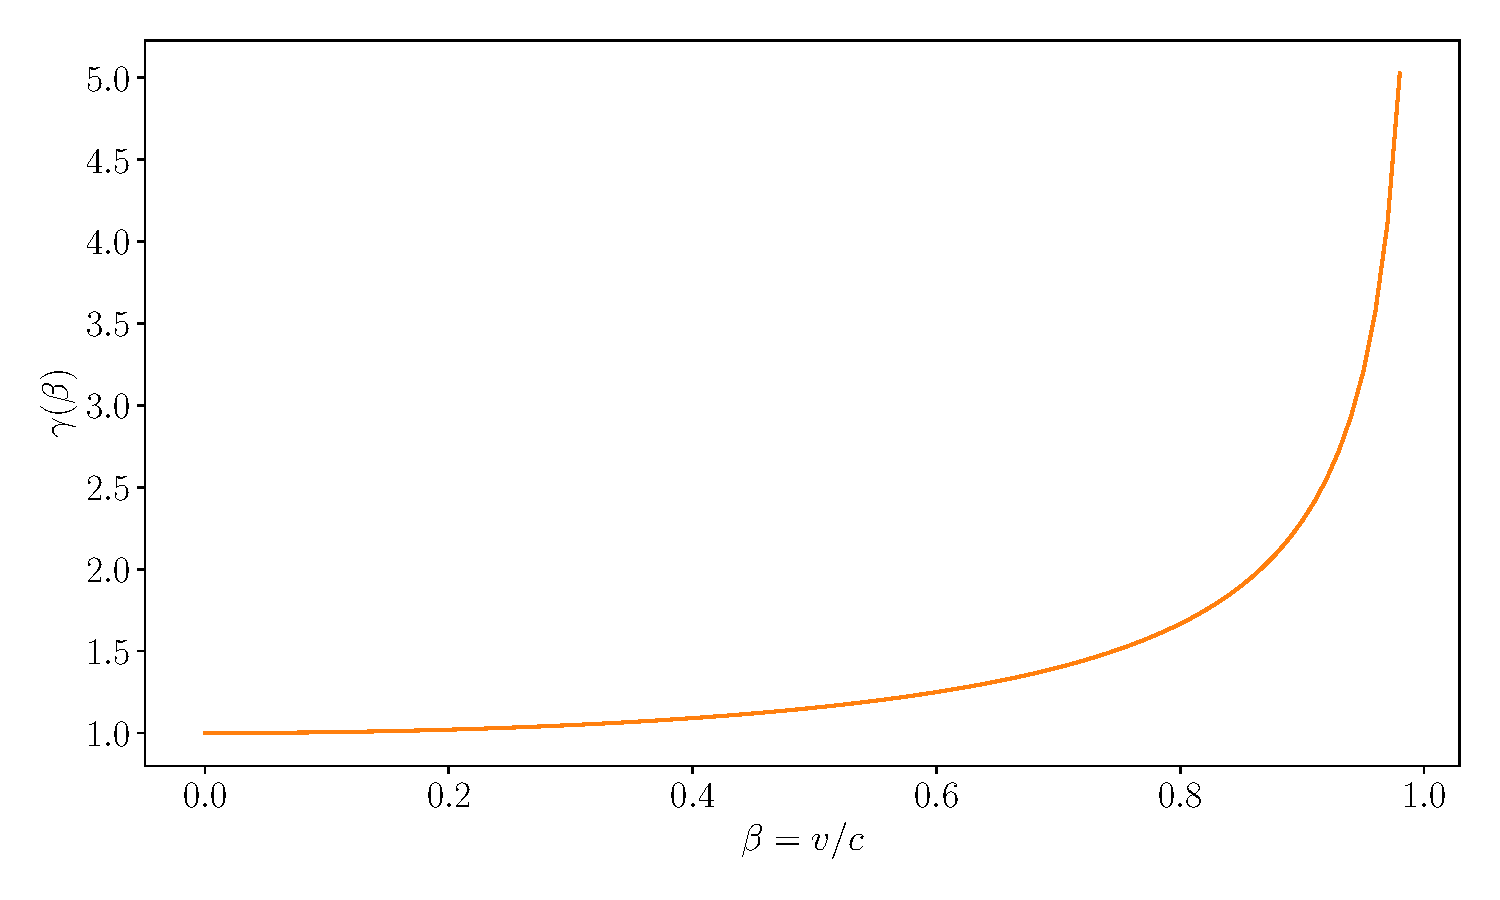
\includegraphics[width=0.9\textwidth]{gamma_factor.pdf}
	
	\caption{Plot of the Lorentz-factor $\gamma = \frac{1}{\sqrt{1 - v^2 / c^2}}$.\\
	Clearly, its effect only becomes significant for speeds which are significant fractions of $c$.}
\end{figure}



		\subsection{Light Cones}
we can visualize Lorentz transformation very nicely in geometric manner/fashion/way


mention future and past light cone


timelike means trajectories are always in light/null cone (Penrose continues to make interesting point on that on page 407: light cones more fundamental than metric) -> does that belong to relativistic dynamics section maybe?


uhhh for spacelike events (equivalent: they do not lie in light cone of other event), their order depends on inertial frame we choose! This is what is meant with causality problems for spacelike events and world lines, cause and effect depend on observer!


talk about spacetime diagrams here -> after all, we will use them in section on clocks (not really anymore) -> better motivation: can visualize effects of Lorentz transformation very nicely

spacetime diagram is basically intersection in light cone, right? Where we only show one spatial dimension


simultaneous events in Minkowski space are one a line parallel to spatial axis; gleichortige (-> equilocal?) events are on a line parallel to time axis



explanation why primed axes are shifted inwards in Minkowski diagrams: we wish to express these axes in the unprimed coordinate system, i.e.~we do not apply the Lorentz transform from unprimed (at rest) to primed (moving with $v$), but rather the inverse one (thus we have to use $-v$ in transformation)



\begin{figure}
	\centering
	
	\begin{tikzpicture}
		% Declare numbers as tikz variables, makes changing very convenient
		\tikzmath{\v = 0.5;}

		% Add basis for diagram
		\spacetimediagram{4}
	
		% Add other observer (one sufficient, for more diagram gets increasingly confusing)
		\addobserver{3}{\v}
	
		%\lightcone{1}{-1}{1}{2}
	
		% Add event in rest frame
		\addevent{0}{2}
		\addevent{2}{2}
	
		% Add same event in moving frame
		\addevent[v=\v, color=blue]{0}{2}
		\addevent[v=\v, color=blue]{2}{2}
	\end{tikzpicture}
	
	\caption{Two events at spacetime points $(0,2), (2,2)$. Red dots show the points with these coordinates in the $(x, ct)$-frame and blue dots show the same coordinates in the $(ct', x')$-frame moving with $v = 0.5 c$.\\
	We can see very nicely how each observer perceives time differently. Events happening simultaneously to both red dots (i.e.~which lie on the line between them at $t = 2$), do \emph{not} happen at $t' = t$, but at $t' = \tau = \sqrt{1 - v^2} \, t$ (which is evident from the fact that the blue dots are at $t' = t$). The same can be said for the moving observer in blue, which sees events at $t = \sqrt{1 - v^2} \, t'$ simultaneous to the blue dots at $t' = 2$.}
\end{figure}



-> introduce spacetime diagrams with multiple observers, can also explain twin paradox very nicely -> but should work before, right?


\begin{ex}[Twin Paradox 2]\label{ex:twin_paradox_2}
As promised, here comes the detailed demonstration of the twin paradox, which has been started in example \ref{ex:twin_paradox_1}. We will discuss the setup shown in figure \ref{fig:twin_paradox}, i.e.~treat one observer at rest (will be commonly referred to as \enquote{unprimed} one) and two observers moving with velocities $v = \pm 0.5 c$ relative to the unprimed observer (these will be called \enquote{primed} and \enquote{double primed}, in accordance with their axis labels in \ref{fig:twin_paradox}).

Our approach will be to compute the roundtrip time needed to go from $S$ to $E$ (i.e.~the time passing on the world line on $ct$ axis) and the time needed to go from $S$ to $T$ to $E$ (i.e.~the time passing on the other world line shown in \ref{fig:twin_paradox}). Each of these quantities will be computed from clocks resting in all three of the inertial frames shown in figure \ref{fig:twin_paradox} (reminder: three are involved due to turning around, rest frame of moving observer changes there).

%the thing that makes things make sense is that all observers agree on the time passing along moving clock, even when measured from their coordinates; after all, from the double primed coordinates we can still look at time passing on clock in primed coordinates and simultaneously passing in rest frame; adding that up, we get the total times and these agree between the frames (good, otherwise we would have problem)

During the process, we have to distinguish between four times: (i) the time $t_{ST}$ passing on the resting clock between $S$ and $T$, (ii) the time $t_{TE}$ passing on the resting clock between $T$ and $E$, (iii) the time $\tau_{ST}$ passing on the moving clock between $S$ and $T$ and (iv) the time $\tau_{TE}$ passing on the moving clock between $T$ and $E$. From that we get the total times for resting and moving clock,
\begin{equation*}
t_{SE} = t_{ST} + t_{TE}
\manyqquad
\tau_{SE} = \tau_{ST} + \tau_{TE} = t'_{ST} + t''_{TE} \, .
\end{equation*}

One final note concerns the velocities involved: the world line is drawn for $v = 0.5 c$ on the way from $S$ to $T$ and $v = -0.5 c$ on the way from $T$ to $E$ (same velocity, different direction), where $v$ is the velocity of the respective moving frame compared to the unprimed, resting one. This implies a relative velocity of $v_2 = \frac{0.5 c + 0.5 c}{1 + 0.5^2} = 0.8 c$ from double primed to primed frame (note that addition of velocities works differently in relativity).

\begin{itemize}
	\item \textbf{Measuring from unprimed coordinates}
	
	Clearly,
	\begin{equation*}
	t_{ST} = 2 = t_{TE}
	\qquad \Leftrightarrow \qquad
	t_{SE} = t_{ST} + t_{TE} = 4
	\end{equation*}
	in arbitrary time units (where one time unit goes by between two grid lines). From that, Minkowski's theorem tells us
	\begin{equation*}
	t'_{SE} = \sqrt{1 - v^2} \, t_{SE} = 3.464 \, .
	\end{equation*}

	Simultaneously, by looking at how much time elapses between the intersection of gray grid lines and the blue $ct'$-axis, one can see that as a rough estimate $t'_{ST} \lesssim 2$. For the exact result, we apply Minkowski's theorem:
	\begin{equation*}
	t'_{ST} = \tau_{ST} = \sqrt{1 - v^2 / c^2} \, t_{ST} = \sqrt{1 - 0.5^2} \cdot 2 = 1.732 \, .
	\end{equation*}
	Applying the same procedure to the double primed coordinates yields
	\begin{equation*}
	t''_{TE} = \tau_{TE} = \sqrt{1 - v^2 / c^2} \, t_{TE} = \sqrt{1 - (-0.5)^2} \cdot 2 = 1.732 = \tau_{ST} \, .
	\end{equation*}
	
	This is because time dilation does not depend on the direction, only on the absolute velocity. Therefore, we can confirm that
	\begin{equation*}
	t_{SE} = t_{ST} + t_{TE} = 4 > \tau_{SE} = \tau_{ST} + \tau_{TE} = 3.464 \, ,
	\end{equation*}
	less time goes by on the moving clock.
	


	\item \textbf{Measuring from primed coordinates}

	While from these coordinates one still sees four time units going by on the roundtrip for the resting observer, i.e.~$t_{SE} = 4$, a rough estimate for the roundtrip time measured by a clock resting in the primed coordinates $ct'$ is $t'_{SE} \gtrsim 4$. More precisely, Minkowski's theorem yields
	\begin{equation*}
	t_{SE} = \sqrt{1 - v^2 / c^2} \, t'_{SE}
	\qquad \Leftrightarrow \qquad
	t'_{SE} = \frac{t_{SE}}{\sqrt{1 - v^2 / c^2}} = \frac{4}{\sqrt{1 - (-0.5)^2}} = 4.619 \, .
	\end{equation*}
	This is a consequence from the mutuality of time dilation, an observer resting in primed coordinates sees the unprimed observer moving at $v = -0.5 c$ and therefore measures more time passing in his own frame.


	However, $t'_{SE}$ is not what a clock in the primed coordinates sees. Instead, 
	\begin{equation*}
	\tau_{SE} = \tau_{ST} + \tau_{TE} = t'_{ST} + t''_{TE}
	\end{equation*}
	as stated before. For $t'_{ST}$, however, we cannot simply use Minkowski's theorem and thus the time
	\begin{equation*}
	\frac{t_{ST}}{\sqrt{1 - v^2 / c^2}} = 2.309 \, ,
	\end{equation*}
	which cannot be quite correct since from the diagram we get the estimate $t'_{ST} \lesssim 3$. This is because the world line is moving with respect to the rest frame of $ct$, so we would only get statements about what is the time as seen from this frame. However, we wish to measure the primed time from the primed coordinates. This requires a Lorentz transformation of the events $S, T, E$:
	\begin{equation*}
	t'_{ST} = t'_T - t'_S = \frac{t_T - \frac{v}{c} x_T}{\sqrt{1 - v^2 / c^2}} - \frac{t_S - \frac{v}{c} x_S}{\sqrt{1 - v^2 / c^2}} = \frac{t_{ST} - \frac{v}{c} x_T}{\sqrt{1 - v^2 / c^2}} = \frac{2 - 0.5 \cdot 1}{\sqrt{1 - 0.5^2}} = 1.732 \, .
	\end{equation*}
	In the same manner, we obtain
	\begin{equation*}
	t'_{TE} = t'_E - t'_T = \frac{t_E - \frac{v}{c} x_E}{\sqrt{1 - v^2 / c^2}} - \frac{t_T - \frac{v}{c} x_T}{\sqrt{1 - v^2 / c^2}} = \frac{t_{TE} + \frac{v}{c} x_T}{\sqrt{1 - v^2 / c^2}} = \frac{2 + 0.5 \cdot 1}{\sqrt{1 - (-0.5)^2}} = 2.887 \, .
	\end{equation*}

	To get $t''_{TE}$, we have to prolong the axes of simultaneity of the primed coordinates and count the number of time units which go by between the intersections of them with $ct''$ (i.e.~the number of intersections with green lines on the way). This yields roughly $t''_{TE} \gtrsim 1.5$ again. For the time passing simultaneously on a clock in primed coordinates, we can read off roughly $t'_{TE} \approx 4$. The correct numbers can be obtained from Minkowski's theorem again:
	\begin{equation*}
	t''_{TE} = \sqrt{1 - (-v_2)^2 / c^2} \, t'_{TE} = \sqrt{1 - (-0.8)^2} \, 2.887 = 1.732 \, .
	\end{equation*}

	All together, the primed observer measures a roundtrip time
	\begin{equation*}
	t'_{SE} = t'_{ST} + t'_{TE} = 4.619 > \tau_{SE} = \tau_{ST} + \tau_{TE} = t'_{ST} + t''_{TE} = 3.464 \, .
	\end{equation*}
	We find the same result that less time has passed on the moving clock. Furthermore, we see that the absolute value for this $\tau_{SE} = t'_{SE}$ and the one computed from Minkowski's theorem in the first calculation agree (because corresponding world line is parallel to $ct$, i.e.~in rest frame). On the other hand, it should not be surprising that the absolute values measured for $\tau_{ST}$ and $\tau_{TE}$ do not agree. After all, they are still measured from different inertial frames and they measure with respect to frames moving with different relative velocities ($\pm 0.5$ for primed; $0.5, 0.8$ for unprimed).

	
	% for v=0.7 c
	%on own clock, six time units go by for roundtrip; however, he agrees that just four go by on resting clock
	
	%on own clock, it is again roughly $3 / 2$ which pass by; on $ct''$ he sees $3 / 2$ passing by as well (way to see that: look at which lines parallel to $x'$ intersect the relevant events, i.e.~starting point and turning point; then look at points where these lines intersect $ct''$ and count number of ticks on $ct''$ between these intersections); in the same manner, we see that four time units pass on $ct$
	
	\item \textbf{Measuring from double primed coordinates}

	Just as before, $t_{SE} = 4$ is measured, while roughly $t''_{SE} \gtrsim 4$ and precisely
	\begin{equation*}
	t''_{SE} = \frac{t_{SE}}{\sqrt{1 - v^2 / c^2}} = \frac{4}{\sqrt{1 - (-0.5)^2}} = 4.619
	\end{equation*}
	are measured by a clock resting in the double primed coordinates. As one can confirm by looking at the result above, this is the same time a clock resting in primed coordinates measures. We expect more of these equal results since the double primed coordinate system is moves with the same relative velocity as the primed one, just in the other direction (sign of velocity is different).

	A rough estimate for $t''_{TE}$ is $t''_{TE} \gtrsim 2$ and the exact result is
	\begin{equation*}
	t''_{TE} = t''_E - t''_T = \frac{t_E - \frac{v}{c} x_E}{\sqrt{1 - v^2 / c^2}} - \frac{t_T - \frac{v}{c} x_T}{\sqrt{1 - v^2 / c^2}} = \frac{t_{TE} + \frac{v}{c} x_T}{\sqrt{1 - v^2 / c^2}} = \frac{2 - 0.5 \cdot 1}{\sqrt{1 - (-0.5)^2}} = 1.732 \, .
	\end{equation*}
	An analogous calculation yields
	\begin{equation*}
	t''_{ST} = t''_T - t''_S = \frac{t_T - \frac{v}{c} x_T}{\sqrt{1 - v^2 / c^2}} - \frac{t_S - \frac{v}{c} x_S}{\sqrt{1 - v^2 / c^2}} = \frac{t_{ST} - \frac{v}{c} x_T}{\sqrt{1 - v^2 / c^2}} = \frac{2 + 0.5 \cdot 1}{\sqrt{1 - 0.5^2}} = 2.887 \, .
	\end{equation*}
	As promised, we get more results that we have already seen when making computations in the primed coordinates, but now they are switched (due to the transition $v \rightarrow -v$).

	Now we wish to compute $t'_{ST}$ and expect the rough estimate $t'_{ST} \gtrsim 1.5$. Indeed, we obtain
	\begin{equation*}
	t'_{ST} = \sqrt{1 - v_2^2 / c^2} \, t'_{TE} = \sqrt{1 - 0.8^2} \, 2.887 = 1.732 \, .
	\end{equation*}
	All in all, the double primed observer measures a roundtrip time
	\begin{equation*}
	t''_{SE} = t''_{ST} + t''_{TE} = 4.619 > \tau_{SE} = \tau_{ST} + \tau_{TE} = t'_{ST} + t''_{TE} = 3.464 \, .
	\end{equation*}
	Once again, these results look very familiar. 
\end{itemize}

A conclusion of these extensive calculations is that physics is not broken, despite the sometimes unintuitive nature of relativity. Although all inertial frames play equal roles, which shows in the mutual slowing of moving clocks, all agree on the effect of time dilation: moving clocks tick slower than resting ones.

It should also be noted that the agreement of all three observers regarding $\tau_{SE}$ is really a coincidence due to the symmetric setup we have chosen -- for other scenarios, e.g.~with unequal velocities on the first and second part of the journey or perhaps even if we assume that $ct$ is not at rest after all (but keeping the relative velocities of primed and unprimed system, i.e.~rotating the whole setup).
\end{ex}

\begin{figure}
	\centering

	\begin{tikzpicture}
		% Declare numbers as tikz variables, makes changing very convenient
		\tikzmath{\vprime = 0.5; \vdoubleprime = -0.5;
				  \tS = -2; \tT = 0;
				  \tE = 2; \xS = 0;
				  \xT = (\tT - \tS) * \vprime; \xE = 0;
				  }  % Note: world line connecting S and T is always parallel to time axis of primed observer, while world line connecting T and E is only parallel to double primed if vprime=-vdoubleprime

		% Add basis for diagram
		\spacetimediagram{4}
	
		% Add other observers
		\addobserver{3}{\vprime}
		\addobserver[xlabel=$x''$, ylabel=$ct''$, color=black!40!green]{3}{\vdoubleprime}

		% Add worldlines of clocks and start, end events
		\addworldline{\xS}{\tS}{\xT}{\tT}  % Resting clock
		\addworldline{\xS}{\tS}{\xT}{\tT}  % Moving clock
		\addworldline{\xT}{\tT}{\xE}{\tE}  % Moving clock

		\addevent[radius=2pt, label=$S$, label placement=right]{\xS}{\tS}  % S
		\addevent[radius=2pt, label=$T$, label placement=right]{\xT}{\tT}  % T
		\addevent[radius=2pt, label=$E$, label placement=right]{\xE}{\tE}  % E
	\end{tikzpicture}

	\caption{Visual explanation of twin paradox. Event $S$ is the starting point, $T$ turning point and $E$ end point. The primed observer has a relative velocity of $v = 0.5 v$ with respect to the unprimed one, while the double primed observer has $v = -0.5 c$.\\
	We can measure times passing between events in a certain frame $\mathcal{O}$ by prolonging the corresponding lines of simultaneity (parallel to spatial axis of $\mathcal{O}$) from event to the time axis of $\mathcal{O}$ and then count the number of time units passing on the time axis between the intersection points. Similarly, we could also prolong them until they intersect the time axis of any other frame $\mathcal{O}'$. In this case, counting the number of time steps passing between the intersection points on the time axis of $\mathcal{O}'$ would yield the time passing for $\mathcal{O}'$, measured from $\mathcal{O}$.}
	\label{fig:twin_paradox}
\end{figure}


\iffalse
{ % Idea was to explain situation from every frame -> does not make things less complicated, thus omitted
\begin{figure}
	\centering

	\begin{tikzpicture}
		% Add basis for diagram
		\spacetimediagram[xlabel=$x'$, ylabel=$ct'$, color=blue]{4}
	
		% Add other observers
		\addobserver[xlabel=$x$, ylabel=$ct$, color=black]{3}{(-1) * 0.5}
		\addobserver[xlabel=$x''$, ylabel=$ct''$, color=black!40!green]{3}{(-1) * 0.8}

		% Add worldlines of clocks and start, end events
		%\draw[red, thick, cm={1/0.866,-0.5/0.866,-0.5/0.866,1/0.866,(0,0)}] (0, -2) -- (0, 2); % Resting clock
		\addworldline[v=-0.5]{0}{-2}{0}{2}
		%\draw[red, thick, cm={1/0.866,-0.5/0.866,-0.5/0.866,1/0.866,(0,0)}] (0, -2) -- (0.5 * 2, 0) -- (0, 2); % Moving clock
		\addworldline[v=-0.5]{0}{-2}{0.5 * 2}{0}
		\addworldline[v=-0.5]{0.5 * 2}{0}{0}{2}
		\addevent[v=-0.5, radius=2pt, label=$S$, label placement=right]{0}{-2}
		\addevent[v=-0.5, radius=2pt, label=$T$, label placement=right]{0.5 * 2}{0}
		\addevent[v=-0.5, radius=2pt, label=$E$, label placement=right]{0}{2}
	\end{tikzpicture}

	\caption{Visual explanation of twin paradox.\\
	We can measure times passing between events in a certain frame by looking at the lines of simultaneity (parallel to spatial axis of this frame), prolonging them from event to time axis of the frame and then count the number of time units passing on the time axis between the intersection points.}
	\label{fig:twin_paradox_prime}
\end{figure}

\begin{figure}
	\centering

	\begin{tikzpicture}
		% Add basis for diagram
		\spacetimediagram[xlabel=$x''$, ylabel=$ct''$, color=black!40!green]{4}
	
		% Add other observers
		\addobserver[xlabel=$x$, ylabel=$ct$, color=black]{3}{0.5}
		\addobserver[xlabel=$x'$, ylabel=$ct'$, color=blue]{3}{0.8}

		% Add worldlines of clocks and start, end events
		\addworldline[v=0.5]{0}{-2}{0}{2}  % Resting clock
		\addworldline[v=0.5]{0}{-2}{0.5 * 2}{0} % Moving clock
		\addworldline[v=0.5]{0.5 * 2}{0}{0}{2}
		\addevent[v=0.5, radius=2pt, label=$S$, label placement=right]{0}{-2}
		\addevent[v=0.5, radius=2pt, label=$T$, label placement=right]{0.5 * 2}{0}
		\addevent[v=0.5, radius=2pt, label=$E$, label placement=right]{0}{2}
	\end{tikzpicture}

	\caption{Visual explanation of twin paradox.\\
	We can measure times passing between events in a certain frame by looking at the lines of simultaneity (parallel to spatial axis of this frame), prolonging them from event to time axis of the frame and then count the number of time units passing on the time axis between the intersection points.}
	\label{fig:twin_paradox_doubleprime}
\end{figure}

}
\fi



\newpage



	\section{Minkowski Space}
Throughout the last sections, we discovered more and more how space and time work in relativity and how they are related. Important contributions to that picture were made by the insights of Einstein regarding synchronization of clocks and Lorentz, who developed a corrected version of the Galilei transform.

It might be clear to the reader that this implies space and time are not independent anymore, but instead have to be treated on the same footing. Historically speaking, however, this final step was not made until Minkowski proposed his viewpoint that physics should take place in a four-dimensional \Def{spacetime}. This unification is an essential part of how the theory of relativity is described in modern literature, in particular because it allows a description in terms of a well-developed mathematical theory -- the theory of manifolds. We will also adopt the usage from now on.


%over the course of the last sections, we saw more and more how space time work in relativity and how they are related; Einstein's insights and Lorentz transform show how clocks work differently than their Newtonian pendants once relativity principle is incorporated, they are not independent anymore; but it is only with the Minkowskian viewpoint that this connection is fully unveiled/completed by uniting them into one spacetime (which goes along with unified mathematical formulation on sound/fond footing)


do mathematical stuff; also mention interpretation of Lorentz transformation as symmetry group stuff (?)





		\subsection{Basic Definitions}
First, it is necessary to state what spacetime is in a formal, mathematical way.


\begin{defi}[Minkowski Space]

4-manifold, points called events; coordinates usually denoted as $\mathbf{\xi} = \mqty(c t \\ \vec{x}) = \mqty(c t \\ x \\ y \\ z)$

events can then be described using 4-vectors $\mathbf{\xi} = \mqty(c t \\ \vec{x}) = \mqty(c t \\ x \\ y \\ z)$ (called \Def{event} from now on) -> but that is point, right? Not vector; we choose to scale time such that all components have the same units; factors of $c$ are kind of nasty in relativity, which is why very often $c$ is set to $1$ (this way, first coordinate is simply time but scaling and computations are still convenient)
\end{defi}



physical way to say things: we want observer-independent statements, for example on spatial distances and time; mathematical: coordinate-independent, invariant notions like distance and metric -> this is why language of manifolds is so convenient: its underlying, mathematical ideas are conceptually equivalent to key physical ideas of relativity



events are now spacetime points, world lines are collections of events and thus curves (can usually be parametrized; parameter with specific normalization is called proper time)


introduce four-velocity as tangent vector; then also state that as of now, we are not able to take norm of it -> motivates metric section



just like coordinate planes with $x-, y-$axis visualize Euclidian space, spacetime diagrams visualize spacetime; although often time-axis versus only one spatial axis; for this reason, they are also commonly called \Def{Minkowski diagrams}



		\subsection{Notes}

turns out there is a very convenient way to formulate what we just learned, in terms of manifolds (where we use coordinates only as a tool, similar to what we require for different inertial frames); will also enable to formulate some properties in a very nice manner

ok, this might be nice: in spacetime diagrams, we see the idea how space and time (which are, as we know now, no separate notions) can be combined into one entity -- describe them as coordinates in one space; this space is called Minkowski space and spacetime diagrams can be seen as a visualization of it; SR is basically which geometry Minkowski space possesses and mathematically, we can describe that in metric; this metric we get from invariant notion we have already seen




\hrule




to be more general than moving with constant speed, let's use the very general definition of how to measure lengths of curves $\gamma(t)$ defined on some interval $I$: $L(\gamma) = \int_I \sqrt{g_{\mu \nu} v^\mu v^\nu} \, dt = \int_I \sqrt{g(v, v)} \, dt$, $v = \gamma'(t)$ ($t$-dependence omitted); this is done using the metric $g$ and generalizing from the example where we subtract spatial coordinates from time yields
\begin{equation}
g = \eta = \mqty(1 & 0 & 0 & 0 \\ 0 & -1 & 0 & 0 \\ 0 & 0 & -1 & 0 \\ 0 & 0 & 0 & -1)
\end{equation}
in basis $\mathbf{\xi} = \mqty(c t \\ \vec{x}) = \mqty(c t \\ x \\ y \\ z)$; this already determines the (pseudo) metric as a tensor because of invariance when changing the basis

the corresponding line element is
\begin{equation}
ds^2 := (ds)^2 = g_{\mu \nu} dx^\mu dx^\nu = c^2 dt^2 - \norm{d\vec{x}}^2 = c^2 dt^2 - dx^2 - dy^2 - dz^2
\end{equation}
where $g_{\mu \nu} = g(\pdv{x^\mu}, \pdv{x^\nu})$


to see equivalence to what was deduced for non-constant speed, we rewrite condition from example \ref{ex:mov_obs}:
\begin{equation*}
c^2 t^2 = c^2 t'^2 - v^2 t'^2 = c^2 t'^2 - \norm{\vec{x}}^2
\end{equation*}
times $t$, distances $\norm{x}$ are nothing but differences from $0$ and for infinitesimal differences, this reads
\begin{equation*}
c^2 dt^2 = c^2 dt'^2 - \norm{d\vec{x}}^2
\end{equation*}
which is nothing but $ds^2$ (is invariant, just like $\tau$); this shows us very cool feature of formalized description, effects like time dilation simply follow from demanding that $ds^2$ or $d\tau^2$ (equivalent) do not depend on the inertial/coordinate system they are measured in, i.e.~$ds^2 = ds'^2$



therefore, we can compute the time elapsed along a world line $\Gamma$ (which is nothing but a curve in Minkowski space) according to
\begin{equation}
\tau = \int d\tau = \frac{1}{c} \int ds
\end{equation}
if the time $t$ in some frame of reference can be measured, the proper time element can be rewritten as:
\begin{equation}
d\tau = \frac{ds}{c} = \frac{\sqrt{ds^2}}{c} = \frac{1}{c} \sqrt{c^2 dt^2 - d\vec{x}^2} = \frac{dt}{c} \sqrt{c^2 - \dv{\vec{x}}{t} \dv{\vec{x}}{t}} = dt \sqrt{1 - \frac{v^2}{c^2}} =: \gamma dt
\end{equation}
where $\gamma$ is the \Def{Lorentz-factor}


if we have some world line $\gamma(\sigma): \sigma \mapsto \qty(t, x, y, z) = \qty(t(\sigma), x(\sigma), y(\sigma), z(\sigma))$ parametrized by a parameter $\sigma \in \qty[a, b]$, we can also compute the proper time using this parametrization:
\begin{equation}
%\tau = \frac{1}{c} \int_\Gamma ds = \frac{1}{c} \int_\Gamma \sqrt{c^2 dt^2 - dx^2 - dy^2 - dz^2} = \frac{1}{c} \int
\tau = \int_\Gamma d\tau = \int_a^b \dv{t}{\sigma} \gamma \, d\sigma = \frac{1}{c} \int_a^b \sqrt{\qty(\dv{t}{\sigma})^2 - \qty(\dv{\vec{x}}{\sigma})^2} \, d\sigma
\end{equation}
should be correct, is just transformation law for integrals... last equality from Dragon, should be equivalent to previous ones (guess it just depends on situation which one is used); this formula is valid for accelerated clocks as well (reduces to the previous one for time difference in case of uniformly moving clock/observer)




		\subsection{Metric \& Inner Product}
We have now seen how physics can be conveniently described using a 4D manifold, which we called spacetime. Points on this manifold are events and we can change coordinates or inertial frames using Lorentz-transformations. Moreover, there are several quantities that can be defined naturally on manifolds, for example curves, vectors, and covectors (maps that take vectors as input). While manifolds do have an additional natural structure, this is given by topology. In physics, however, we are also interested in statements concerned with distances between events and to measure them we need additional structure. More specifically, we have to specify a metric that will allow measuring distances, as well as norms of vectors via the induced inner product.


Mathematically, metrics are objects called tensors and they have the convenient property that they are invariant under coordinate changes. Therefore, distances are physical statements because they do not depend on the inertial frame we compute them on. In the tradition of invariant quantities that have been encountered so far, we may guess that the metric will be related to light in some way. From the universality of the speed if light $c$, distances $s$ are equivalent to times $t$ for light, $s = c t$. Because of that, a natural measure for distances is the time elapsed on a clock, i.e.~the geometric structure of Minkowski space is determined by Minkowski's theorem \ref{thm:minkowski_moving_clocks}. Instead of denoting time with the usual variable $t$, we will now switch to the \Def{proper time} $\tau$ since the time elapsed a clock between events $(0, 0, 0, 0)$ and $(ct, x, y, z)$ is
\begin{equation}\label{eq:proper_time_uniform}
\eqbox{
\tau = \sqrt{1 - \frac{v^2}{c^2}} \, t = \sqrt{1 - \qty(\frac{x}{ct})^2 - \qty(\frac{y}{ct})^2 - \qty(\frac{z}{ct})^2} \, t = \sqrt{t^2 - (x^2 + y^2 + z^2) / c^2}
}
\end{equation}
This depends on the trajectory taken by the clock/corresponding observer (more specifically, on the uniform velocity $v$), but will in general not be equal to $t$, which is the time measured simultaneously by a clock resting in the corresponding frame. In example \ref{ex:twin_paradox_2} we have seen how observers do not necessarily agree on times $t$ their own clocks measure between two events, but they do agree on times measured by a clock moving on a trajectory connecting these two events.


What was denoted with $\tau$ in equation \eqref{eq:proper_time_uniform}, in reality is a difference $\Delta \tau$ of proper times (just measured with respect to $\tau = 0$), and the same is true for the coordinates $(ct, x, y, z)$. Making these differences infinitesimally small, i.e.~$\Delta \rightarrow d$, we obtain the infinitesimal distance or \Def{proper time element} (strictly mathematically: \Def{line element})\footnote{We adopt the common notation $dx^2 := (dx)^2$.}
\begin{equation}
\eqbox{
d\tau^2 = dt^2 - \frac{dx^2 + dy^2 + dz^2}{c^2}
} \, .
\end{equation}
This implies the following \Def{proper line element}
\begin{equation}
\eqbox{
ds^2 = c^2 d\tau^2 = c^2 dt^2 - dx^2 - dy^2 - dz^2
}
\end{equation}
and corresponding \Def{proper distance} $s = c \tau$ between events. This specific form of the line element immediately gives us the components of the \Def{Minkowski metric} $\eta$, which can be conveniently arranged in a matrix
\begin{equation}
\eqbox{
\eta = \mqty(1 & 0 & 0 & 0 \\ 0 & -1 & 0 & 0 \\ 0 & 0 & -1 & 0 \\ 0 & 0 & 0 & -1)
} \, .
\end{equation}
At this point, we shall make a remark regarding the signs: in principle, we could have chosen $\eta$ to have only one minus (in the time component) since only the proper time is constrained by physical observations, while the proper distance could equally well be defined as $ds^2 = - c^2 d\tau^2$. There are good arguments for both conventions, but I personally find it more natural to keep the signs when going from times to distances, which is why the $(+, -, -, -)$-convention is adopted here.\\


-> maybe mention general formula for proper time here (with integral)?


From the metric, one can infer statements about the geometry of Minkowski space. In Euclidian space, points of constant distance $s$ lie on a circle around the origin, which is determined by the equation $s^2 = x^2 + y^2 + z^2$. In Minkowski space, events of equal distance lie on a hyperboloid of constant proper times $\tau$ and are determined by
\begin{equation}\label{eq:eichhyperbel}
\eqbox{
c^2 \tau^2 = c^2 t^2 - x^2 - y^2 - z^2
} \, .
\end{equation}
Setting $c \tau = 1$ yields a hyperbola, whose intersection with time axes in spacetime diagrams determines the \enquote{length of one time unit} (figure \ref{fig:minkowski_with_eichhyperbel}).


\begin{figure}
	\centering

	\begin{tikzpicture}
		% Add basis for diagram
		\spacetimediagram{4}
	
		% Add other observers
		\addobserver{2}{0.5}
		%\addobserver{2}{0.7}

		% Add eichhyperbel. From $1 = c^2 t^2 - x^2$ we get parametrization $(x, ct) = (x, \sqrt{1 + x^2})$
		\draw[domain=-4:4, smooth, variable=\x, color=black!30!green] plot ({\x}, {sqrt(1 + \x * \x)});
	\end{tikzpicture}

	\caption{Plot of the curve fulfilling $1 = c^2 t^2 - x^2 - y^2 - z^2$ (green), along with two inertial frames (rest frame in black and frame moving with $v = 0.5 c$ relative to resting one in blue).\\
	As we can see, this yields same time steps as Lorentz transform, hyperbola intersects $ct'$-axis perfectly at $c t' = 1$ (as it should).}
	\label{fig:minkowski_with_eichhyperbel}
\end{figure}


One final note concerns an alternative derivation of the metric. It is also based on the relativity principle, but instead of constructing clocks etc.~explicitly, it uses that light propagates as a spherical wave with velocity $c$. Writing this equation in multiple inertial frames yields
\begin{equation}
c^2 t^2 = x^2 + y^2 + z^2 \; \text{ and } \; c^2 t'^2 = x'^2 + y'^2 + z'^2 \qquad \Leftrightarrow \qquad c^2 t^2 - x^2 - y^2 - z^2 \overset{!}{=} c^2 t'^2 - x'^2 - y'^2 - z'^2 \, .
\end{equation}
by the equivalence principle. This points to the invariant proper distance we have called $s$ (which vanishes for light). At the same time, it explains the ambiguity in overall sign because we can get the same physics no matter which sign is used in $ds^2$ (only the sign in $d\tau^2$ is fixed, but this can be adjusted by defining $ds^2 = \pm c^2 d\tau^2$, respectively).



		\paragraph{Inner Product}

for a world line $\Gamma$ with tangent vector $\underline{t}$, we call it timelike etc if $\eta(\underline{t}, \underline{t}) = \eval{ds^2}_\Gamma$ has certain value (turns out that this value is constant throughout curve)


To end this subsection, we note that the line element allows the following, very compact, definition.
\begin{defi}[Timelike, Lightlike, Spacelike]
A world line $\Gamma$ is called
\begin{itemize}
\item \Def{timelike}, if $ds^2> 0 \; \Leftrightarrow \; c > v$ along $\Gamma$


\item \Def{null/lightlike}, if $ds^2 = 0 \; \Leftrightarrow \; c = v$ along $\Gamma$


\item \Def{spacelike}, if $ds^2 < 0 \; \Leftrightarrow \; c < v$ along $\Gamma$
\end{itemize}
\end{defi}
We already knew the terms before, but now they can be restated in a more formal way, which adds to the intuitive definition from before.


more thoughts inspired by Dragon script: we have seen how to measure time $\tau$ that elapses for observer; we can formalize this into scalar product which takes two tangent vectors as input; the value of this inner product tells us about the properties of the world line we compute the tangent vectors for, if it is timelike/lightlike/spacelike






		\subsection{Lorentz Transformations 2}
-> I think introducing them before Minkowski section still makes sense because they were there before description as manifolds; but now, they get more general meaning as change of coordinates/charts etc, so we look at them again

-> after metric is nice, then we can present mathematical viewpoint; do not change norm of four-vector; also note that they admit group structure, i.e.~note properties here; maybe even introduce rapidity and note connection of Lie group and Lie algebra? But not elaborate on this

maybe just note that Lorentz transformation = change of coordinates/charts (which is corresponding term in language of manifolds); one condition to obtain them is by demanding norm of four-vector does not change (ahh, might be confusing because I think Nolting refers to this kind of in Euclidian space; what he calls norm is really proper time passing on clock which moves from origin to point, isn't it? Would make sense to demand this better stay the same after transformation after we have put so much effort into invariant definition) -> I like this, but does not fit before introduction of norm; so maybe make subsection on transformations after metric?



now that we know how times from different frames of reference are related, we may ask for more general relations between them


when interpreting Minkowski space as a manifold and working with coordinates/charts $\xi$, we know the results should be independent of $\xi$; in particular, that means they hold in other charts as well and changing coordinates is an important part; the basis changes even have a distinct name, \Def{Lorentz transformation}; this is basically group theory due to the symmetries that Minkowski space possesses (known from logic and experiments) ?right?




\newpage



	\section{Relativistic Dynamics}
we have dependence on world line of our distance measure; this is nothing unusual in mathematical theory of metric spaces, but it raises an important physical question: what is the preferred trajectory of particles, i.e.~what is the time that usually elapses for them? Turns out that it is extremal proper time (minimal for us, depends on sign convention of metric, right?), which yields straight lines.


idea: new transformation law means we have new dynamics; these can be formulated conveniently using points and vectors in Minkowski space; talk about four-momentum and forces etc.

$4$-momentum is related to velocity, that is tangent vector; therefore, we can also compute inner product for it



		\subsection{Four-velocity and Four-momentum}
four-velocity: using chain rule, we can write $U^\alpha = \dv{x^\alpha}{\tau} = \dv{t}{\tau} \dv{x^\alpha}{t} =: \gamma (c, \vec{v})$ in general; this $\gamma = \dv{t}{\tau} = \pdv{t}{\tau}$ then depends on the metric, it is the (negative of, depends on convention that is chosen) component $g_{tt}$; for the Minkowski metric in SR (where only uniform velocities occur), we can further simplify this by using $d\tau^2 = ds^2 / c^2 = (c^2 dt^2 - dx^2 - dy^2 - dz^2) / c^2 = dt^2 (1 - \dv{x^\alpha}{t} \dv{x^\alpha}{t} / c^2) =: dt^2 / \gamma^2$; this $\gamma$ us negligible for many problems, only has significant effects if $v \approx c$ (which is why it is does not show up in daily life)



redshift leads to higher energy, but frequency also changes such that all in all speed of light remains constant (might be wrong this way, but heard something like that)




		\subsection{Acceleration}%{Accelerated Observers} % GR is next chapter, maybe this name more accurate
using the generalization we just made, we can also deal with accelerations, i.e.~non-uniform movement; this is easier (or at least more straightforward) to do than intuitive version, at least for now



we have seen how to compute proper times in special relativity, the formula could be broken down to 
\begin{equation}
\tau = \int d\tau = \frac{1}{c} \int ds = \frac{1}{c} \int \sqrt{g_{\mu \nu} v^\mu v^\nu} \, dt
\end{equation}

in fact, this formula also holds for $v = v(t)$, i.e.~when a time-dependent velocity and thus acceleration is present (we can compute dynamics); this is because it does not involve absolute differences like $x - x'$, but infinitesimal ones $dx$ along the whole path, so changes in $v$ are incorporated automatically; however, we have to use other metrics in this case and general relativity presents a general way to compute the metric



good start I think: \url{https://de.wikipedia.org/wiki/Zeitdilatation#Bewegung_mit_konstanter_Beschleunigung}




for non-uniform velocity, connection procedure does not work between macroscopic events anymore (because getting distance from velocity is not multiplication, now integration), but only infinitesimally (equivalent: just like we have to integrate velocity for distance, we have to integrate for travel time of light; since time = distance for light -> nice visualization: rectification of curve, works perfect for straight line, but if changing derivative comes into play, not perfect anymore, have to go to infinitesimal distances for that); motivation for $d\tau$





\end{document}